%%%%%%%%%%%%%%%%%%%%%%%%%%%%%%%%%%%%%%%%%
% The Legrand Orange Book
% LaTeX Template
% Version 2.4 (26/09/2018)
%
% This template was downloaded from:
% http://www.LaTeXTemplates.com
%
% Original author:
% Mathias Legrand (legrand.mathias@gmail.com) with modifications by:
% Vel (vel@latextemplates.com)
%
% License:
% CC BY-NC-SA 3.0 (http://creativecommons.org/licenses/by-nc-sa/3.0/)
%
% Compiling this template:
% This template uses biber for its bibliography and makeindex for its index.
% When you first open the template, compile it from the command line with the 
% commands below to make sure your LaTeX distribution is configured correctly:
%
% 1) pdflatex main
% 2) makeindex main.idx -s StyleInd.ist
% 3) biber main
% 4) pdflatex main x 2
%
% After this, when you wish to update the bibliography/index use the appropriate
% command above and make sure to compile with pdflatex several times 
% afterwards to propagate your changes to the document.
%
% This template also uses a number of packages which may need to be
% updated to the newest versions for the template to compile. It is strongly
% recommended you update your LaTeX distribution if you have any
% compilation errors.
%
% Important note:
% Chapter heading images should have a 2:1 width:height ratio,
% e.g. 920px width and 460px height.
%
%%%%%%%%%%%%%%%%%%%%%%%%%%%%%%%%%%%%%%%%%

%%%%%%%%%%%%%%%%%%%%%%%%%%%%%%%%%%%%%%%%%
% 附加说明:
% 1、本模板源文件如上所述,经修改用于发布笔记的release版本
% 2、
%%%%%%%%%%%%%%%%%%%%%%%%%%%%%%%%%%%%%%%%%
%----------------------------------------------------------------------------------------
%	PACKAGES AND OTHER DOCUMENT CONFIGURATIONS
%----------------------------------------------------------------------------------------

\documentclass[11pt,fleqn]{book} % Default font size and left-justified equations

%%%%%%%%%%%%%%%%%%%%%%%%%%%%%%%%%%%%%%%%%
% The Legrand Orange Book
% Structural Definitions File
% Version 2.1 (26/09/2018)
%
% Original author:
% Mathias Legrand (legrand.mathias@gmail.com) with modifications by:
% Vel (vel@latextemplates.com)
% 
% This file was downloaded from:
% http://www.LaTeXTemplates.com
%
% License:
% CC BY-NC-SA 3.0 (http://creativecommons.org/licenses/by-nc-sa/3.0/)
%
%%%%%%%%%%%%%%%%%%%%%%%%%%%%%%%%%%%%%%%%%

%----------------------------------------------------------------------------------------
%	VARIOUS REQUIRED PACKAGES AND CONFIGURATIONS
%----------------------------------------------------------------------------------------

\usepackage{graphicx} % Required for including pictures
\graphicspath{{Pictures/}} % Specifies the directory where pictures are stored

\usepackage{lipsum} % Inserts dummy text

\usepackage{tikz} % Required for drawing custom shapes

\usepackage[english]{babel} % English language/hyphenation

\usepackage{enumitem} % Customize lists
\setlist{nolistsep} % Reduce spacing between bullet points and numbered lists

\usepackage{booktabs} % Required for nicer horizontal rules in tables

\usepackage{xcolor} % Required for specifying colors by name
\definecolor{ocre}{RGB}{243,102,25} % Define the orange color used for highlighting throughout the book

%----------------------------------------------------------------------------------------
%	MARGINS
%----------------------------------------------------------------------------------------

\usepackage{geometry} % Required for adjusting page dimensions and margins

\geometry{
	paper=a4paper, % Paper size, change to letterpaper for US letter size
	top=3cm, % Top margin
	bottom=3cm, % Bottom margin
	left=3cm, % Left margin
	right=3cm, % Right margin
	headheight=14pt, % Header height
	footskip=1.4cm, % Space from the bottom margin to the baseline of the footer
	headsep=10pt, % Space from the top margin to the baseline of the header
	%showframe, % Uncomment to show how the type block is set on the page
}

%----------------------------------------------------------------------------------------
%	FONTS
%----------------------------------------------------------------------------------------

\usepackage{avant} % Use the Avantgarde font for headings
%\usepackage{times} % Use the Times font for headings
\usepackage{mathptmx} % Use the Adobe Times Roman as the default text font together with math symbols from the Sym­bol, Chancery and Com­puter Modern fonts

\usepackage{microtype} % Slightly tweak font spacing for aesthetics
\usepackage[utf8]{inputenc} % Required for including letters with accents
\usepackage[T1]{fontenc} % Use 8-bit encoding that has 256 glyphs

%----------------------------------------------------------------------------------------
%	BIBLIOGRAPHY AND INDEX
%----------------------------------------------------------------------------------------

\usepackage[style=numeric,citestyle=numeric,sorting=nyt,sortcites=true,autopunct=true,babel=hyphen,hyperref=true,abbreviate=false,backref=true,backend=biber]{biblatex}
\addbibresource{bibliography.bib} % BibTeX bibliography file
\defbibheading{bibempty}{}

\usepackage{calc} % For simpler calculation - used for spacing the index letter headings correctly
\usepackage{makeidx} % Required to make an index
\makeindex % Tells LaTeX to create the files required for indexing

%----------------------------------------------------------------------------------------
%	MAIN TABLE OF CONTENTS
%----------------------------------------------------------------------------------------

\usepackage{titletoc} % Required for manipulating the table of contents

\contentsmargin{0cm} % Removes the default margin

% Part text styling (this is mostly taken care of in the PART HEADINGS section of this file)
\titlecontents{part}
	[0cm] % Left indentation
	{\addvspace{20pt}\bfseries} % Spacing and font options for parts
	{}
	{}
	{}

% Chapter text styling
\titlecontents{chapter}
	[1.25cm] % Left indentation
	{\addvspace{12pt}\large\sffamily\bfseries} % Spacing and font options for chapters
	{\color{ocre!60}\contentslabel[\Large\thecontentslabel]{1.25cm}\color{ocre}} % Formatting of numbered sections of this type
	{\color{ocre}} % Formatting of numberless sections of this type
	{\color{ocre!60}\normalsize\;\titlerule*[.5pc]{.}\;\thecontentspage} % Formatting of the filler to the right of the heading and the page number

% Section text styling
\titlecontents{section}
	[1.25cm] % Left indentation
	{\addvspace{3pt}\sffamily\bfseries} % Spacing and font options for sections
	{\contentslabel[\thecontentslabel]{1.25cm}} % Formatting of numbered sections of this type
	{} % Formatting of numberless sections of this type
	{\hfill\color{black}\thecontentspage} % Formatting of the filler to the right of the heading and the page number

% Subsection text styling
\titlecontents{subsection}
	[1.25cm] % Left indentation
	{\addvspace{1pt}\sffamily\small} % Spacing and font options for subsections
	{\contentslabel[\thecontentslabel]{1.25cm}} % Formatting of numbered sections of this type
	{} % Formatting of numberless sections of this type
	{\ \titlerule*[.5pc]{.}\;\thecontentspage} % Formatting of the filler to the right of the heading and the page number

% Figure text styling
\titlecontents{figure}
	[1.25cm] % Left indentation
	{\addvspace{1pt}\sffamily\small} % Spacing and font options for figures
	{\thecontentslabel\hspace*{1em}} % Formatting of numbered sections of this type
	{} % Formatting of numberless sections of this type
	{\ \titlerule*[.5pc]{.}\;\thecontentspage} % Formatting of the filler to the right of the heading and the page number

% Table text styling
\titlecontents{table}
	[1.25cm] % Left indentation
	{\addvspace{1pt}\sffamily\small} % Spacing and font options for tables
	{\thecontentslabel\hspace*{1em}} % Formatting of numbered sections of this type
	{} % Formatting of numberless sections of this type
	{\ \titlerule*[.5pc]{.}\;\thecontentspage} % Formatting of the filler to the right of the heading and the page number

%----------------------------------------------------------------------------------------
%	MINI TABLE OF CONTENTS IN PART HEADS
%----------------------------------------------------------------------------------------

% Chapter text styling
\titlecontents{lchapter}
	[0em] % Left indentation
	{\addvspace{15pt}\large\sffamily\bfseries} % Spacing and font options for chapters
	{\color{ocre}\contentslabel[\Large\thecontentslabel]{1.25cm}\color{ocre}} % Chapter number
	{}  
	{\color{ocre}\normalsize\sffamily\bfseries\;\titlerule*[.5pc]{.}\;\thecontentspage} % Page number

% Section text styling
\titlecontents{lsection}
	[0em] % Left indentation
	{\sffamily\small} % Spacing and font options for sections
	{\contentslabel[\thecontentslabel]{1.25cm}} % Section number
	{}
	{}

% Subsection text styling (note these aren't shown by default, display them by searchings this file for tocdepth and reading the commented text)
\titlecontents{lsubsection}
	[.5em] % Left indentation
	{\sffamily\footnotesize} % Spacing and font options for subsections
	{\contentslabel[\thecontentslabel]{1.25cm}}
	{}
	{}

%----------------------------------------------------------------------------------------
%	HEADERS AND FOOTERS
%----------------------------------------------------------------------------------------

\usepackage{fancyhdr} % Required for header and footer configuration

\pagestyle{fancy} % Enable the custom headers and footers

\renewcommand{\chaptermark}[1]{\markboth{\sffamily\normalsize\bfseries\chaptername\ \thechapter.\ #1}{}} % Styling for the current chapter in the header
\renewcommand{\sectionmark}[1]{\markright{\sffamily\normalsize\thesection\hspace{5pt}#1}{}} % Styling for the current section in the header

\fancyhf{} % Clear default headers and footers
\fancyhead[LE,RO]{\sffamily\normalsize\thepage} % Styling for the page number in the header
\fancyhead[LO]{\rightmark} % Print the nearest section name on the left side of odd pages
\fancyhead[RE]{\leftmark} % Print the current chapter name on the right side of even pages
%\fancyfoot[C]{\thepage} % Uncomment to include a footer

\renewcommand{\headrulewidth}{0.5pt} % Thickness of the rule under the header

\fancypagestyle{plain}{% Style for when a plain pagestyle is specified
	\fancyhead{}\renewcommand{\headrulewidth}{0pt}%
}

% Removes the header from odd empty pages at the end of chapters
\makeatletter
\renewcommand{\cleardoublepage}{
\clearpage\ifodd\c@page\else
\hbox{}
\vspace*{\fill}
\thispagestyle{empty}
\newpage
\fi}

%----------------------------------------------------------------------------------------
%	THEOREM STYLES
%----------------------------------------------------------------------------------------

\usepackage{amsmath,amsfonts,amssymb,amsthm} % For math equations, theorems, symbols, etc

\newcommand{\intoo}[2]{\mathopen{]}#1\,;#2\mathclose{[}}
\newcommand{\ud}{\mathop{\mathrm{{}d}}\mathopen{}}
\newcommand{\intff}[2]{\mathopen{[}#1\,;#2\mathclose{]}}
\renewcommand{\qedsymbol}{$\blacksquare$}
\newtheorem{notation}{Notation}[chapter]

% Boxed/framed environments
\newtheoremstyle{ocrenumbox}% Theorem style name
{0pt}% Space above
{0pt}% Space below
{\normalfont}% Body font
{}% Indent amount
{\small\bf\sffamily\color{ocre}}% Theorem head font
{\;}% Punctuation after theorem head
{0.25em}% Space after theorem head
{\small\sffamily\color{ocre}\thmname{#1}\nobreakspace\thmnumber{\@ifnotempty{#1}{}\@upn{#2}}% Theorem text (e.g. Theorem 2.1)
\thmnote{\nobreakspace\the\thm@notefont\sffamily\bfseries\color{black}---\nobreakspace#3.}} % Optional theorem note

\newtheoremstyle{blacknumex}% Theorem style name
{5pt}% Space above
{5pt}% Space below
{\normalfont}% Body font
{} % Indent amount
{\small\bf\sffamily}% Theorem head font
{\;}% Punctuation after theorem head
{0.25em}% Space after theorem head
{\small\sffamily{\tiny\ensuremath{\blacksquare}}\nobreakspace\thmname{#1}\nobreakspace\thmnumber{\@ifnotempty{#1}{}\@upn{#2}}% Theorem text (e.g. Theorem 2.1)
\thmnote{\nobreakspace\the\thm@notefont\sffamily\bfseries---\nobreakspace#3.}}% Optional theorem note

\newtheoremstyle{blacknumbox} % Theorem style name
{0pt}% Space above
{0pt}% Space below
{\normalfont}% Body font
{}% Indent amount
{\small\bf\sffamily}% Theorem head font
{\;}% Punctuation after theorem head
{0.25em}% Space after theorem head
{\small\sffamily\thmname{#1}\nobreakspace\thmnumber{\@ifnotempty{#1}{}\@upn{#2}}% Theorem text (e.g. Theorem 2.1)
\thmnote{\nobreakspace\the\thm@notefont\sffamily\bfseries---\nobreakspace#3.}}% Optional theorem note

% Non-boxed/non-framed environments
\newtheoremstyle{ocrenum}% Theorem style name
{5pt}% Space above
{5pt}% Space below
{\normalfont}% Body font
{}% Indent amount
{\small\bf\sffamily\color{ocre}}% Theorem head font
{\;}% Punctuation after theorem head
{0.25em}% Space after theorem head
{\small\sffamily\color{ocre}\thmname{#1}\nobreakspace\thmnumber{\@ifnotempty{#1}{}\@upn{#2}}% Theorem text (e.g. Theorem 2.1)
\thmnote{\nobreakspace\the\thm@notefont\sffamily\bfseries\color{black}---\nobreakspace#3.}} % Optional theorem note
\makeatother

% Defines the theorem text style for each type of theorem to one of the three styles above
\newcounter{dummy} 
\numberwithin{dummy}{section}
\theoremstyle{ocrenumbox}
\newtheorem{theoremeT}[dummy]{Theorem}
\newtheorem{problem}{Problem}[chapter]
\newtheorem{exerciseT}{Exercise}[chapter]
\theoremstyle{blacknumex}
\newtheorem{exampleT}{Example}[chapter]
\theoremstyle{blacknumbox}
\newtheorem{vocabulary}{Vocabulary}[chapter]
\newtheorem{definitionT}{Definition}[section]
\newtheorem{corollaryT}[dummy]{Corollary}
\theoremstyle{ocrenum}
\newtheorem{proposition}[dummy]{Proposition}

%----------------------------------------------------------------------------------------
%	DEFINITION OF COLORED BOXES
%----------------------------------------------------------------------------------------

\RequirePackage[framemethod=default]{mdframed} % Required for creating the theorem, definition, exercise and corollary boxes

% Theorem box
\newmdenv[skipabove=7pt,
skipbelow=7pt,
backgroundcolor=black!5,
linecolor=ocre,
innerleftmargin=5pt,
innerrightmargin=5pt,
innertopmargin=5pt,
leftmargin=0cm,
rightmargin=0cm,
innerbottommargin=5pt]{tBox}

% Exercise box	  
\newmdenv[skipabove=7pt,
skipbelow=7pt,
rightline=false,
leftline=true,
topline=false,
bottomline=false,
backgroundcolor=ocre!10,
linecolor=ocre,
innerleftmargin=5pt,
innerrightmargin=5pt,
innertopmargin=5pt,
innerbottommargin=5pt,
leftmargin=0cm,
rightmargin=0cm,
linewidth=4pt]{eBox}	

% Definition box
\newmdenv[skipabove=7pt,
skipbelow=7pt,
rightline=false,
leftline=true,
topline=false,
bottomline=false,
linecolor=ocre,
innerleftmargin=5pt,
innerrightmargin=5pt,
innertopmargin=0pt,
leftmargin=0cm,
rightmargin=0cm,
linewidth=4pt,
innerbottommargin=0pt]{dBox}	

% Corollary box
\newmdenv[skipabove=7pt,
skipbelow=7pt,
rightline=false,
leftline=true,
topline=false,
bottomline=false,
linecolor=gray,
backgroundcolor=black!5,
innerleftmargin=5pt,
innerrightmargin=5pt,
innertopmargin=5pt,
leftmargin=0cm,
rightmargin=0cm,
linewidth=4pt,
innerbottommargin=5pt]{cBox}

% Creates an environment for each type of theorem and assigns it a theorem text style from the "Theorem Styles" section above and a colored box from above
\newenvironment{theorem}{\begin{tBox}\begin{theoremeT}}{\end{theoremeT}\end{tBox}}
\newenvironment{exercise}{\begin{eBox}\begin{exerciseT}}{\hfill{\color{ocre}\tiny\ensuremath{\blacksquare}}\end{exerciseT}\end{eBox}}				  
\newenvironment{definition}{\begin{dBox}\begin{definitionT}}{\end{definitionT}\end{dBox}}	
\newenvironment{example}{\begin{exampleT}}{\hfill{\tiny\ensuremath{\blacksquare}}\end{exampleT}}		
\newenvironment{corollary}{\begin{cBox}\begin{corollaryT}}{\end{corollaryT}\end{cBox}}	

%----------------------------------------------------------------------------------------
%	REMARK ENVIRONMENT
%----------------------------------------------------------------------------------------

\newenvironment{remark}{\par\vspace{10pt}\small % Vertical white space above the remark and smaller font size
\begin{list}{}{
\leftmargin=35pt % Indentation on the left
\rightmargin=25pt}\item\ignorespaces % Indentation on the right
\makebox[-2.5pt]{\begin{tikzpicture}[overlay]
\node[draw=ocre!60,line width=1pt,circle,fill=ocre!25,font=\sffamily\bfseries,inner sep=2pt,outer sep=0pt] at (-15pt,0pt){\textcolor{ocre}{R}};\end{tikzpicture}} % Orange R in a circle
\advance\baselineskip -1pt}{\end{list}\vskip5pt} % Tighter line spacing and white space after remark

%----------------------------------------------------------------------------------------
%	SECTION NUMBERING IN THE MARGIN
%----------------------------------------------------------------------------------------

\makeatletter
\renewcommand{\@seccntformat}[1]{\llap{\textcolor{ocre}{\csname the#1\endcsname}\hspace{1em}}}                    
\renewcommand{\section}{\@startsection{section}{1}{\z@}
{-4ex \@plus -1ex \@minus -.4ex}
{1ex \@plus.2ex }
{\normalfont\large\sffamily\bfseries}}
\renewcommand{\subsection}{\@startsection {subsection}{2}{\z@}
{-3ex \@plus -0.1ex \@minus -.4ex}
{0.5ex \@plus.2ex }
{\normalfont\sffamily\bfseries}}
\renewcommand{\subsubsection}{\@startsection {subsubsection}{3}{\z@}
{-2ex \@plus -0.1ex \@minus -.2ex}
{.2ex \@plus.2ex }
{\normalfont\small\sffamily\bfseries}}                        
\renewcommand\paragraph{\@startsection{paragraph}{4}{\z@}
{-2ex \@plus-.2ex \@minus .2ex}
{.1ex}
{\normalfont\small\sffamily\bfseries}}

%----------------------------------------------------------------------------------------
%	PART HEADINGS
%----------------------------------------------------------------------------------------

% Numbered part in the table of contents
\newcommand{\@mypartnumtocformat}[2]{%
	\setlength\fboxsep{0pt}%
	\noindent\colorbox{ocre!20}{\strut\parbox[c][.7cm]{\ecart}{\color{ocre!70}\Large\sffamily\bfseries\centering#1}}\hskip\esp\colorbox{ocre!40}{\strut\parbox[c][.7cm]{\linewidth-\ecart-\esp}{\Large\sffamily\centering#2}}%
}

% Unnumbered part in the table of contents
\newcommand{\@myparttocformat}[1]{%
	\setlength\fboxsep{0pt}%
	\noindent\colorbox{ocre!40}{\strut\parbox[c][.7cm]{\linewidth}{\Large\sffamily\centering#1}}%
}

\newlength\esp
\setlength\esp{4pt}
\newlength\ecart
\setlength\ecart{1.2cm-\esp}
\newcommand{\thepartimage}{}%
\newcommand{\partimage}[1]{\renewcommand{\thepartimage}{#1}}%
\def\@part[#1]#2{%
\ifnum \c@secnumdepth >-2\relax%
\refstepcounter{part}%
\addcontentsline{toc}{part}{\texorpdfstring{\protect\@mypartnumtocformat{\thepart}{#1}}{\partname~\thepart\ ---\ #1}}
\else%
\addcontentsline{toc}{part}{\texorpdfstring{\protect\@myparttocformat{#1}}{#1}}%
\fi%
\startcontents%
\markboth{}{}%
{\thispagestyle{empty}%
\begin{tikzpicture}[remember picture,overlay]%
\node at (current page.north west){\begin{tikzpicture}[remember picture,overlay]%	
\fill[ocre!20](0cm,0cm) rectangle (\paperwidth,-\paperheight);
\node[anchor=north] at (4cm,-3.25cm){\color{ocre!40}\fontsize{220}{100}\sffamily\bfseries\thepart}; 
\node[anchor=south east] at (\paperwidth-1cm,-\paperheight+1cm){\parbox[t][][t]{8.5cm}{
\printcontents{l}{0}{\setcounter{tocdepth}{0}}% The depth to which the Part mini table of contents displays headings; 0 for chapters only, 1 for chapters and sections and 2 for chapters, sections and subsections
}};
\node[anchor=north east] at (\paperwidth-1.5cm,-3.25cm){\parbox[t][][t]{15cm}{\strut\raggedleft\color{white}\fontsize{30}{30}\sffamily\bfseries#2}};
\end{tikzpicture}};
\end{tikzpicture}}%
\@endpart}
\def\@spart#1{%
\startcontents%
\phantomsection
{\thispagestyle{empty}%
\begin{tikzpicture}[remember picture,overlay]%
\node at (current page.north west){\begin{tikzpicture}[remember picture,overlay]%	
\fill[ocre!20](0cm,0cm) rectangle (\paperwidth,-\paperheight);
\node[anchor=north east] at (\paperwidth-1.5cm,-3.25cm){\parbox[t][][t]{15cm}{\strut\raggedleft\color{white}\fontsize{30}{30}\sffamily\bfseries#1}};
\end{tikzpicture}};
\end{tikzpicture}}
\addcontentsline{toc}{part}{\texorpdfstring{%
\setlength\fboxsep{0pt}%
\noindent\protect\colorbox{ocre!40}{\strut\protect\parbox[c][.7cm]{\linewidth}{\Large\sffamily\protect\centering #1\quad\mbox{}}}}{#1}}%
\@endpart}
\def\@endpart{\vfil\newpage
\if@twoside
\if@openright
\null
\thispagestyle{empty}%
\newpage
\fi
\fi
\if@tempswa
\twocolumn
\fi}

%----------------------------------------------------------------------------------------
%	CHAPTER HEADINGS
%----------------------------------------------------------------------------------------

% A switch to conditionally include a picture, implemented by Christian Hupfer
\newif\ifusechapterimage
\usechapterimagetrue
\newcommand{\thechapterimage}{}%
\newcommand{\chapterimage}[1]{\ifusechapterimage\renewcommand{\thechapterimage}{#1}\fi}%
\newcommand{\autodot}{.}
\def\@makechapterhead#1{%
{\parindent \z@ \raggedright \normalfont
\ifnum \c@secnumdepth >\m@ne
\if@mainmatter
\begin{tikzpicture}[remember picture,overlay]
\node at (current page.north west)
{\begin{tikzpicture}[remember picture,overlay]
\node[anchor=north west,inner sep=0pt] at (0,0) {\ifusechapterimage\includegraphics[width=\paperwidth]{\thechapterimage}\fi};
\draw[anchor=west] (\Gm@lmargin,-9cm) node [line width=2pt,rounded corners=15pt,draw=ocre,fill=white,fill opacity=0.5,inner sep=15pt]{\strut\makebox[22cm]{}};
\draw[anchor=west] (\Gm@lmargin+.3cm,-9cm) node {\huge\sffamily\bfseries\color{black}\thechapter\autodot~#1\strut};
\end{tikzpicture}};
\end{tikzpicture}
\else
\begin{tikzpicture}[remember picture,overlay]
\node at (current page.north west)
{\begin{tikzpicture}[remember picture,overlay]
\node[anchor=north west,inner sep=0pt] at (0,0) {\ifusechapterimage\includegraphics[width=\paperwidth]{\thechapterimage}\fi};
\draw[anchor=west] (\Gm@lmargin,-9cm) node [line width=2pt,rounded corners=15pt,draw=ocre,fill=white,fill opacity=0.5,inner sep=15pt]{\strut\makebox[22cm]{}};
\draw[anchor=west] (\Gm@lmargin+.3cm,-9cm) node {\huge\sffamily\bfseries\color{black}#1\strut};
\end{tikzpicture}};
\end{tikzpicture}
\fi\fi\par\vspace*{270\p@}}}

%-------------------------------------------

\def\@makeschapterhead#1{%
\begin{tikzpicture}[remember picture,overlay]
\node at (current page.north west)
{\begin{tikzpicture}[remember picture,overlay]
\node[anchor=north west,inner sep=0pt] at (0,0) {\ifusechapterimage\includegraphics[width=\paperwidth]{\thechapterimage}\fi};
\draw[anchor=west] (\Gm@lmargin,-9cm) node [line width=2pt,rounded corners=15pt,draw=ocre,fill=white,fill opacity=0.5,inner sep=15pt]{\strut\makebox[22cm]{}};
\draw[anchor=west] (\Gm@lmargin+.3cm,-9cm) node {\huge\sffamily\bfseries\color{black}#1\strut};
\end{tikzpicture}};
\end{tikzpicture}
\par\vspace*{270\p@}}
\makeatother

%----------------------------------------------------------------------------------------
%	LINKS
%----------------------------------------------------------------------------------------

\usepackage{hyperref}
\hypersetup{hidelinks,backref=true,pagebackref=true,hyperindex=true,colorlinks=false,breaklinks=true,urlcolor=ocre,bookmarks=true,bookmarksopen=false}

\usepackage{bookmark}
\bookmarksetup{
open,
numbered,
addtohook={%
\ifnum\bookmarkget{level}=0 % chapter
\bookmarksetup{bold}%
\fi
\ifnum\bookmarkget{level}=-1 % part
\bookmarksetup{color=ocre,bold}%
\fi
}
}
 % Insert the commands.tex file which contains the majority of the structure behind the template

%\hypersetup{pdftitle={Title},pdfauthor={Author}} % Uncomment and fill out to include PDF metadata for the author and title of the book

%----------------------------------------------------------------------------------------

% 添加显示中文的部分
\usepackage[UTF8]{ctex}
% 一些数学符号的包
\usepackage{esint}
\usepackage{mathrsfs}
\newcommand{\gt}{\textgreater}
\newcommand{\lt}{\textless}

\begin{document}

%----------------------------------------------------------------------------------------
%	TITLE PAGE
%----------------------------------------------------------------------------------------

%% 注意!这里需要修改的内容有标题,子标题和作者名
\begingroup
\thispagestyle{empty} % Suppress headers and footers on the title page
\begin{tikzpicture}[remember picture,overlay]
\node[inner sep=0pt] (background) at (current page.center) {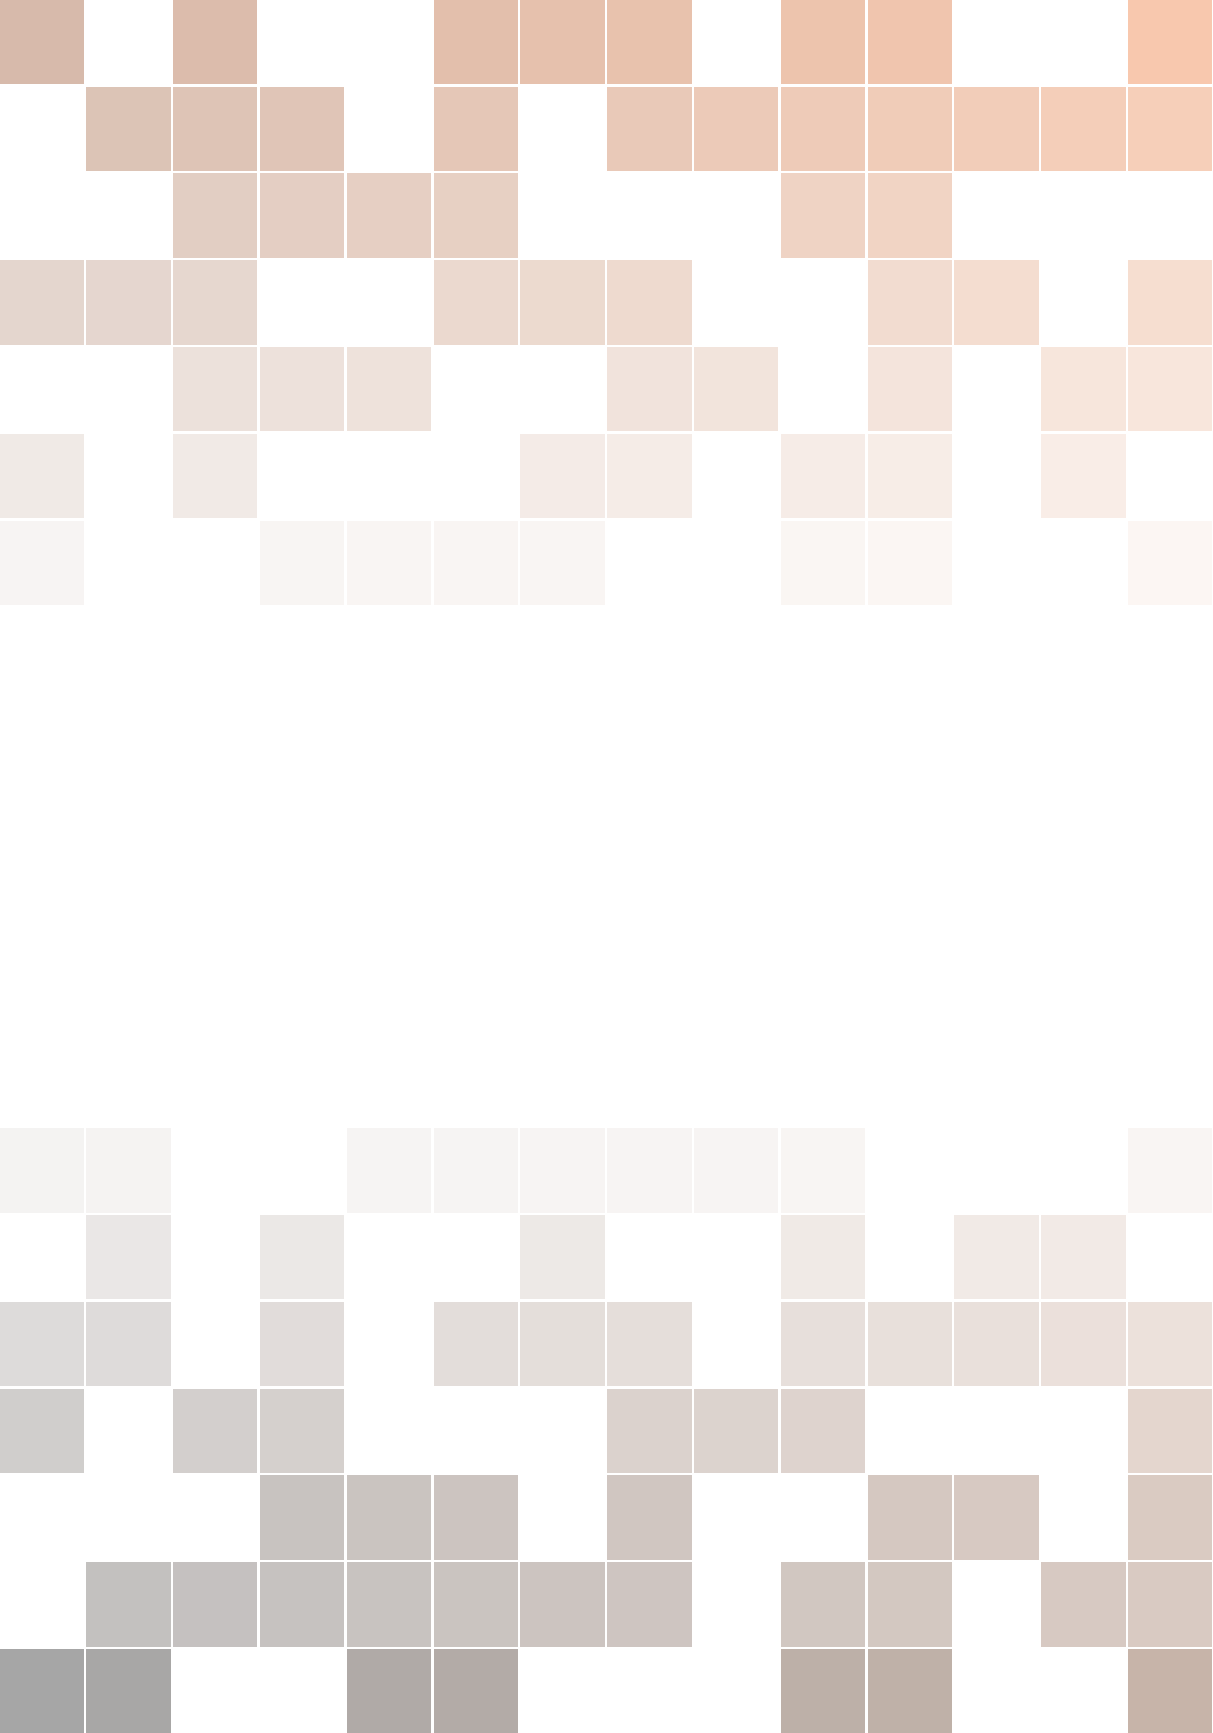
\includegraphics[width=\paperwidth]{background.pdf}};
\draw (current page.center) node [fill=ocre!30!white,fill opacity=0.6,text opacity=1,inner sep=1cm]{\Huge\centering\bfseries\sffamily\parbox[c][][t]{\paperwidth}{\centering 知识点笔记 \\[15pt] % Book title
{\Large 信号系统}\\[20pt] % Subtitle
{\huge Delta1037}}}; % Author name
\end{tikzpicture}
\vfill
\endgroup

%----------------------------------------------------------------------------------------
%	COPYRIGHT PAGE
%----------------------------------------------------------------------------------------

\newpage
~\vfill
\thispagestyle{empty}

\noindent Copyright \copyright\ 2022 Delta1037\\ % Copyright notice

\noindent \textsc{Published by Self}\\ % Publisher

\noindent \textsc{web: www.delta1037.cn}\\ % URL

\noindent \textsc{mail: geniusrabbit@qq.com}\\ % URL

\noindent Licensed under the Creative Commons Attribution-NonCommercial 4.0 Unported License (the ``License''). You may not use this file except in compliance with the License. You may obtain a copy of the License at \url{https://creativecommons.org/licenses/by-nc-sa/4.0/}. Unless required by applicable law or agreed to in writing, software distributed under the License is distributed on an \textsc{``as is'' basis, without warranties or conditions of any kind}, either express or implied. See the License for the specific language governing permissions and limitations under the License.\\ % License information, replace this with your own license (if any)

\noindent \textit{First printing, January 2022} % Printing/edition date

%----------------------------------------------------------------------------------------
%	TABLE OF CONTENTS
%----------------------------------------------------------------------------------------

%\usechapterimagefalse % If you don't want to include a chapter image, use this to toggle images off - it can be enabled later with \usechapterimagetrue

\chapterimage{chapter_head_1.pdf} % Table of contents heading image

\pagestyle{empty} % Disable headers and footers for the following pages

\tableofcontents % Print the table of contents itself

\cleardoublepage % Forces the first chapter to start on an odd page so it's on the right side of the book

\pagestyle{fancy} % Enable headers and footers again

% 对于自动转换部分的说明
% 1、按照chapter对知识点进行分类
% 2、每一个知识点构建成一个section
% 3、一个知识点里如果包含子内容,构建成subsection
% 4、index构建成索引
%%%%%%%%%%%%%%%%%%%%%%%%%%%%%%%%%%%%%%%%%%%%%%%%%%%%%%%%%%%%%%%%%%%%%%%%%%%%%%%%%%%%%%%%%
%----------------------------------------------------------------------------------------
%	PART 1 信号系统
%----------------------------------------------------------------------------------------
\part{信号系统}
%----------------------------------------------------------------------------------------
%	CHAPTER 1 信号系统
%----------------------------------------------------------------------------------------
\chapterimage{chapter_head_2.pdf}
\chapter{信号系统}

\section{时域信号绘图}\index{时域信号绘图}



\subsection{绘制连续信号时域波形}\index{时域信号绘图!绘制连续信号时域波形}

1、横坐标的坐标标识为$t$,纵坐标标识看题目

2、冲激大小用括号加数字表示(表示冲激的强度),负冲激括号里也是正值(因为冲激强度只能为正)

注意:在对含有冲激的图像进行尺度变换时,冲激的大小也会跟着变化

注意:图像在间断点处也有连线(整个图像与$x$轴之间没有间断的地方)

备注:用闭式表达式表示图像时,自变量为$t$,有一次写成了$x$(具体自变量是什么参考题目)



\subsection{绘制离散信号时域波形}\index{时域信号绘图!绘制离散信号时域波形}

1、横坐标的坐标标识为$n$

2、纵坐标轴有没有都可以(如果题目有图形,可以参考题目是怎么画的)

3、端点用圆点表示,非等高的地方标注纵坐标的大小



\subsection{绘制时域波形的奇部和偶部}\index{时域信号绘图!绘制时域波形的奇部和偶部}

1、偶信号:y轴对称的点取平均值放右边,0处不变

2、奇信号:y轴对称的点右边减左边,取平均值,放右边;0处为0

3、对称:将求解后的右边的值按照就行对称到左边

注意:计算端点值,进行验证



\subsection{图形的变换与组合}\index{时域信号绘图!图形的变换与组合}

1、图形变换方式:时移,伸缩,反转(正向变换:(化简成$\alpha(x + \beta)$的形式)先伸缩和反转$\alpha$,再时移$\beta$;逆向变换:先做变量替换,再做正向变换)

2、图形组合方式:加减,求导(注意:连续信号求导时可能会产生冲激信号,看信号与$x$轴之间或者信号本身是否有间断的点)

注意:对特殊点(边界点,信号转折点)进行代入验证



注意波形图的要点:横坐标标注、端点值标注,端点标注

注意:复序列可以将实部和虚部分别表示成两个序列

\section{频域信号绘图}\index{频域信号绘图}



\subsection{连续周期信号的幅度频谱与相位频谱:(条线形式)(双边谱和单边谱)(对比:周期信号傅里叶变换频域是脉冲形式)}\index{频域信号绘图!连续周期信号的幅度频谱与相位频谱:(条线形式)(双边谱和单边谱)(对比:周期信号傅里叶变换频域是脉冲形式)}

1、将周期函数化简为指数信号和的形式$f(t)=\sum_{n=-\infty}^{\infty} F_{n} \mathrm{e}^{\mathrm{j} n \Omega t}$(傅里叶级数的形式)

2、频谱的横坐标为$n \Omega$,纵坐标为$|F_n|$,$\varphi_{n}$(分别时对应$F_n$的模和相位)

3、每一个指数信号的$n \Omega$部分对应为横坐标相应位置(傅里叶级数的$k$值与基波频率$\omega_0$相乘等于一个特定的$\omega$位置的幅度或者相位)

4、按照指数信号的系数求解幅度和相位

注意:如果是绘制单边谱,将函数化为标准傅里叶级数三角函数形式$f(t)=\frac{A_{0}}{2}+\sum_{n=1}^{\infty} A_{n} \cos \left(n \Omega t+\varphi_{n}\right)$,0位置的值为$\frac{A_{0}}{2}$(注意不是$A_{0}$,$A_{0}$是两倍的实际的直流分量)

单双边谱转换:从单边谱转为双边谱,除直流分量外(0位置的值),幅值减半,相位关于原点对称(实信号的傅里叶级数系数的共轭对称性);相应也可以从双边谱转换为单边谱(单双边转换过程中直流分量的幅度是不发生改变的)



\subsection{连续周期信号的傅里叶变换图:(冲激形式)(称为时域信号的频谱)}\index{频域信号绘图!连续周期信号的傅里叶变换图:(冲激形式)(称为时域信号的频谱)}

1、求解周期信号的傅里叶变换(冲激序列形式)

2、绘制各个点的冲激,注意冲激的表示方法



\subsection{离散傅里叶变换图}\index{频域信号绘图!离散傅里叶变换图}

1、图像在间断点是封闭的(间断点有垂线连接)

2、图像是关于$2\pi$是周期的



注意绘图要点:横坐标标注、端点值标注,端点标注

\section{信号性质之奇偶性}\index{信号性质之奇偶性}

1、奇信号的序列和为0(时域信号大小的总和)

2、奇信号与偶信号乘积为奇信号(用定义证明)

3、信号的每一项的平方和等于其奇奇部分的每一项平方和加上偶数部分的每一项的平方和(利用2和展开平方证明)

备注:对连续信号也成立

\section{信号性质之周期性}\index{信号性质之周期性}



\subsection{周期性判断与计算}\index{信号性质之周期性!周期性判断与计算}

1、使用定义判断周期性(特别是异形函数,自变量带平方的)

2、两个信号和:信号周期是两个信号周期的最小公倍数(对于连续信号,周期最小公倍数除以任一个周期的结果不是有理数则不是周期的;对于离散信号,两个整数周期一定有最小公倍数且是整数)

3、代入周期值判断(适用于选择题):根据周期的定义式,将选项代入,并代入$t=0$到定义式中,判断定义式是否成立



\subsection{通过时不变系统后的周期性}\index{信号性质之周期性!通过时不变系统后的周期性}

1、时不变的输入输出周期性:对于时不变的系统,如果输入是周期的,输出也是周期的(时不变的特性)(也可以将周期信号表示为频谱函数的形式来证明)

2、输入非周期,输出可能是周期:可以冲过冲激序列将输入函数扩增成全域内的函数;或者将输入函数中周期比值为无理数的其中一部分抹掉(按照无理数部分的频率特征构造系统的频率响应),使剩余的部分的周期有有理数公比

总结:对于LTI,输入是周期,输出一定是周期;输入是非周期,输出可能是周期



\subsection{信号伸缩变换后的周期性:(连续)}\index{信号性质之周期性!信号伸缩变换后的周期性:(连续)}

1、连续信号伸缩不会改变周期性,伸缩前后周期性一致,但是周期不同



\subsection{信号伸缩变换后的周期性:(离散)}\index{信号性质之周期性!信号伸缩变换后的周期性:(离散)}

1、原信号是周期的,对信号进行抽取和插值之后与原信号周期性一致(周期的计算注意区分之前周期的奇偶性(N为奇数时,可认为是多个周期合并再进行抽取操作))

2、抽取和插值之后的信号是周期的,原信号与信号进行抽取和插值之后的周期性一致不一定一致,离散信号的抽取之后是周期的不代表抽取前是周期的(可能抹掉了一些非周期特性),但是离散信号的插值之后是周期的代表插值之前是周期的

\section{系统的其它性质}\index{系统的其它性质}



\subsection{记忆性}\index{系统的其它性质!记忆性}

1、定义:系统的输出仅取决于该时刻的输入

2、证明:找特殊值,证明某个时间的信号取决于之前的输入

3、样例:累加器(或称为相加器)、延迟单元(都与之前的输入有关)

问题:对于与之后输入相关的是记忆性吗?答:是<奥本海姆 信号系统 第二版 P29 1.6.1 末尾>



\subsection{时不变}\index{系统的其它性质!时不变}

1、先时移再经过系统与先经过系统再时移进行对比,如果一样就是时不变的,如果不一样就是时变的

注意:理解先时移再经过系统,先时移是以原信号($x(t),x[n]$)为基础时移后再代入系统的(在系统外进行时移),不是基于系统中的输入信号(类似于$x(-t),x[-n]$之类的)直接时移的



\subsection{稳定性}\index{系统的其它性质!稳定性}

1、输入有界时输出也有界:设有界输入,判断输出是否是无界的(反证法)

2、LTI系统稳定:单位冲激响应的模在整个域上积分为有限值→稳定LTI(单位脉冲响应的模在整个域上求和为有限值→稳定LTI)

3、收敛域判断:连续系统收敛域包含$jw$轴;离散系统收敛域包含单位圆

4、$H(s)$有理式表示中,如果分母中缺少$s^0$项,则系统一定不稳定



\subsection{因果性}\index{系统的其它性质!因果性}

1、输出不早于输入:当前的输出只能与当前和过去输入有关,即使以未来的判断条件也不行(表达式中任何一处早于输入都不行)(注意:因果性只看输入和输出信号,不关注其它的因式)

2、LTI系统因果:当$t<0$时,$h(t)=0$(离散下,$n<0$时,$h[n]=0$),即具有初始松弛条件

3、其它判断条件:物理可以实现一定是因果的(连续 AND 离散);系统可以由微分方程表示,一定是因果的(连续);系统可以由差分方程表示,不一定是因果的(离散);系统可以由框图表示,不一定是因果的(连续 AND 离散)

4、$H(z)$的收敛域中,如果收敛域不包括无穷,则系统非因果

5、当$H(z)$与已知的信号相乘时,两者的收敛域需要有交集,此时可以推断出系统是因果的(推导过程示例:$H(z)$有两个极点$1/4$和$1/2$,没有明确说明收敛域,所以此时收敛域有三种情况,$X(z)$的收敛域为$|z| \gt 1$,所以此时两者相乘必须有交集,可以得到$H(z)$的收敛域为$|z| \gt 1/2$,也就得到了系统是因果系统)

6、一般对于未特别说明是非因果系统的,默认是因果系统(该条可以否定3和5,即高于3和5)

注意:对于级数$\sum_{i=m}^{n}$表示的输入输出关系的信号,级数上限可能小于下限($m>n$)



\subsection{可逆性}\index{系统的其它性质!可逆性}

1、预判断条件:$x(t)$是否有损值(逆时无法恢复)(损失类型:损失奇部或者偶部、求导损失常数部分、平方损失负数部分、忽略部分$x(t)$的值)

2、预判断条件:$x(t)$是否有多对一的情况(逆变换时无法区分)(损失类型:三角函数)

3、判断:可逆性判断时举反例,两个不同的输入对应同一个输出(输入可以取常数信号)(逆时无法区分的:找输入输出关系图上水平线上的两点输入即可)

\section{判断系统性质}\index{判断系统性质}



\subsection{常见的性质判断特征}\index{判断系统性质!常见的性质判断特征}

1、输入输出关系式带有非常系数的:线性、时变的

2、输入函数变量带有放缩变换的:线性、时变的(注意理解先时移再经过系统)、非因果的

3、输入函数变量带有负常系数的:时变的(注意理解先时移再经过系统,先时移是以原信号($x(t),x[n]$)为基础时移后再代入系统的,不是基于系统中的输入信号(类似于$x(-t),x[-n]$之类的)直接时移的)

4、系统转换函数的定义域与时间相关(非与输入相关):时变的(先经过系统后延时时定义域变了;先延时后经过系统时定义域没有变)(备注:如果定义域是和输入函数相关的(输入函数乘常系数,且变量无放缩),就是非时变的)

5、含有对数运算:非线性,不稳定(因为靠近y轴的地方虽然x是有限的,但是输出是无限的)

6、含有输入信号的高次方运算:非线性



\subsection{性质判断的注意点}\index{判断系统性质!性质判断的注意点}

1、对于输入信号自变量有放大系数(系数小于1)的信号:注意正值部分的记忆性;注意负值部分的非因果性(对于缩小的信号与上述相反)

2、使用导数定义时,注意Δx是可正可负的,正值会导致非因果

3、做时变和线性判断时,若定义域与$x(t)$相关,则分段范围需要与$x(t)$同步变换;定义域中的所有包含$t$的(包括$x(t)$中的$t$)需要与$y(t)$中的$t$同步变化(备注:对于离散信号也是如此)

4、对于未明确定义的信号取偶部:利用偶部表示公式($Ev\{x(t)\}=\frac{x(t)+x(-t)}{2}$)(将$x(t)/x[n]$代入公式即可,即直接令$t=-t/n=-n$,不改变其它的部分)

5、对于复杂的函数可以举反例进行说明

注意:如果是分段函数则注意范围表示是否变换

\section{单位冲激(脉冲)与单位阶跃}\index{单位冲激(脉冲)与单位阶跃}



\subsection{时域中表示}\index{单位冲激(脉冲)与单位阶跃!时域中表示}

1、连续:单位冲激信号和单位阶跃信号

2、离散:单位脉冲序列和单位阶跃序列



\subsection{频域中表示}\index{单位冲激(脉冲)与单位阶跃!频域中表示}

1、连续:单位冲激响应和单位阶跃响应

2、离散:单位脉冲响应和单位阶跃响应



\subsection{恒等系统:(输入输出为常数倍关系,并不是一倍)(注意与信号失真的条件区分)}\index{单位冲激(脉冲)与单位阶跃!恒等系统:(输入输出为常数倍关系,并不是一倍)(注意与信号失真的条件区分)}

1、离散恒等系统性质:$h[n]=k\delta[n]$

2、连续恒等系统性质:$h(t)=k\delta(t)$



\subsection{单位脉冲(冲激)响应与单位阶跃响应的关系}\index{单位冲激(脉冲)与单位阶跃!单位脉冲(冲激)响应与单位阶跃响应的关系}

1、单位脉冲与单位阶跃响应:$h[n]=s[n]-s[n-1]$(推导:$\delta[n]=u[n]-u[n-1]=u[n]-u[n]*\delta[n-1]$,两边同时与系统信号卷积即可得出上述结论);$s[n]=\sum_{k=0}^{\infty}h[n-k]$(由$u[n]=\sum_{k=0}^{\infty}\delta[n-k]$两边同时与输入卷积得到)(单位阶跃函数是单位冲激函数的累加积分)

2、单位冲激与单位阶跃响应:$h(t) = \frac {ds(t)}{t}$(单位冲激是单位阶跃的导数)(如果冲激函数没有突变类型的点(冲激),则说明阶跃信号是连续的)(拉氏变换中会添加或者消去0处的极点)

注意:真分式展开之后,每一项都是真分式,不包含常数项或者$s$的多项式,意味着冲激响应在$t=0$处不包含冲激函数及其导数



\subsection{冲激函数的运算性质}\index{单位冲激(脉冲)与单位阶跃!冲激函数的运算性质}

1、尺度性质:$\delta(at)=\frac{1}{|a|}\delta(t)$,$\delta(at-t_0)=\frac{1}{|a|}\delta(t-\frac{t_0}{a})$(⇒ 冲激函数是偶函数)(如果遇到带有非最简形式的冲激函数,都要化简成最简形式)

2、抽取性质:$x[n] \delta\left[n-n_{0}\right]=x\left[n_{0}\right] \delta\left[n-n_{0}\right]$,$\int_{-\infty}^{\infty} f(t) \delta\left(t-t_{0}\right) d t=f\left(t_{0}\right)$,$f(t) \delta\left(t-t_{0}\right)=f\left(t_{0}\right) \delta\left(t-t_{0}\right)$

3、导数(冲激偶)性质:$\int_{-\infty}^{\infty} \delta^{\prime}(t) d t=0$,$\int_{-\infty}^{t} \delta^{\prime}(\tau) d \tau=\delta(t)$,$\int_{-\infty}^{\infty} f(t) \delta^{\prime}(t) d t=-f^{\prime}(0)$,$\int_{-\infty}^{\infty} f(t) \delta^{\prime}\left(t-t_{0}\right) d t=-f^{\prime}\left(t_{0}\right)$,$f(t) \delta^{\prime}(t)=f(0) \delta^{\prime}(t)-f^{\prime}(0) \delta(t)$(推导:$(f(0)\cdot \delta(t))^\prime =(f(t)\cdot \delta(t))^\prime = f^\prime(x)\delta(t)+f(t)\delta^\prime(t) \Rightarrow f(t) \delta^{\prime}(t)=f(0) \delta^{\prime}(t)-f^{\prime}(0) \delta(t)$,即由乘积函数求导来推导)

4、冲激函数化简:若$f(t)=0$有$n$个互不相等的实数单根$t_{i}(i=1,2, \cdots, n)$,即$f^{\prime}\left(t_{i}\right) \neq 0$,则有$\delta[f(t)]=\sum_{i=1}^{n} \frac{1}{\left|f^{\prime}\left(t_{i}\right)\right|} \delta\left[\left(t-t_{i}\right)\right]$(具体的证明见page页面)(如果有重实根怎么办?放弃考研)

5、冲激函数与阶跃函数的关系:$\delta(t)= u^{\prime}(t)$

6、冲激偶的积分:冲激偶绝对值的积分是不存在的,即冲激偶不是绝对可积的;冲激偶不加绝对值的积分是0

备注:冲激函数只有积分才能消去(另外注意积分时注意积分点是否在积分范围内)

\section{信号平均功率和总能量}\index{信号平均功率和总能量}



\subsection{连续信号}\index{信号平均功率和总能量!连续信号}

1、平均功率公式:$P_{\infty} \triangleq \lim_{T \rightarrow \infty} \frac{1}{2 T} \int_{-T}^{T}|x(t)|^{2} d t$(无穷区间上函数模平方的积分,除以区间长度)(范围中T取无穷极限,范围从-T→ T)(备注:信号的平均功率可以与帕萨瓦尔定律相关联)

2、总能量公式:$E_{\infty} \triangleq \lim_{T \rightarrow \infty} \int_{-T}^{T}|x(t)|^{2} d t=\int_{-\infty}^{+\infty}|x(t)|^{2} d t$(无穷区间上函数模平方的积分)(范围中T取无穷极限,范围从-T→ T)



\subsection{离散信号}\index{信号平均功率和总能量!离散信号}

1、平均功率公式:$P_{\infty} \triangleq \lim_{N \rightarrow \infty} \frac{1}{2 N+1} \sum_{n=-N}^{+N}|x[n]|^{2}$(无穷区间上序列模平方的求和,除以区间长度)(范围中N取无穷极限,范围从-N→ N,项数一共是2N+1项)(备注:信号的平均功率可以与帕萨瓦尔定律相关联)

2、总能量公式:$E_{\infty} \triangleq \lim_{N \rightarrow \infty} \sum_{n=-N}^{+N}|x[n]|^{2}=\sum_{n=-\infty}^{+\infty}|x[n]|^{2}$(无穷区间上序列模平方的求和)(范围中N取无穷极限,范围从-N→ N,项数一共是2N+1项)



\subsection{信号分类}\index{信号平均功率和总能量!信号分类}

1、信号能量有限,平均功率为0(能量信号)

2、平均功率有限,信号能量无穷(功率信号)

2、信号能量无穷,平均功率无穷



\subsection{能量的计算}\index{信号平均功率和总能量!能量的计算}

1、对于能量的计算,首先想到帕萨瓦尔定理

\section{信号范围问题}\index{信号范围问题}



\subsection{根据指定信号值求解时间或者序列范围:<小蓝书 P6 1-2>}\index{信号范围问题!根据指定信号值求解时间或者序列范围:<小蓝书 P6 1-2>}

1、根据已有的方程确定

2、可以采用特殊值代入进行验证

注意:考虑无穷处的值是否满足



\subsection{输入$x[n]$界定值和输出$y[n]$界定值的关系}\index{信号范围问题!输入$x[n]$界定值和输出$y[n]$界定值的关系}

0、假设输入界定值为$B$,输出界定值为$C$(界定值是信号的范围小于该界定值,其它情况立即推)

1、通过输入与输出的关系,估算输出的用输入表示的界定值(用B表示的式子)

2、由于输出界定值是最接近输出的,所以C应该小于等于上述估算的用B表示的式子(注意取等号的条件,对输入的值的要求)

\section{离散信号的基波频率问题}\index{离散信号的基波频率问题}

<小蓝书 P27 1-26 1-27>(写的太复杂,理解即可)

0、假设:信号为$x[n]=e^{jm(2\pi / N)n}$

1、结论:$gcd(m,N)$是$m$和$N$中的最大公约数,则离散信号$x[n]=e^{jm(2\pi / N)n}$的基波周期为$N_0 = N / gcd(m,N)$

2、理解:对于信号$x_1[n]=e^{j2(2\pi / 3)n}$和$x_2[n]=e^{j(2\pi / 3)n}$,按照以上结论,这两个信号的基波周期都是3,区别在于$x_1[n]$的角频率比$x_2[n]$的角频率变化的快,当$x_1[n]$的角频率变化再快一些,变成$x_3[n]=e^{j3(2\pi / 3)n}$,这时$x_3[n]=e^{j(2\pi)n}$,基波周期变成了1,当$x_1[n]$的角频率变化再快一些,变成$x_4[n]=e^{j4(2\pi / 3)n}$,这时基波周期又变成了3(类似于人眼的只能按照指定频率扫描,当看风扇转动时,看到有扇叶静止的时候,可能是频率又轮转回来了)

3、应用:对于一连续信号$x(t)=e^{jw_0t}$,基波频率是$w_0$,基波周期$T_0$是$2\pi / w_0$,对该离散信号进行$T$的等间隔取样,即$x[n] = x(nT) = e^{jw_0nT}$,可以使用周期的定义(设周期是$N$,使用周期的定义进行证明,试着证一下)来证明只有$T/T_0$是有理数时,$x[n]$才是周期的,设周期是$N$,即$\frac{T}{T_0}=\frac{p}{q}$,其中$p$和$q$都是有理数(注意$\frac{p}{q}$不一定是最简形式),则$x[n] = e^{jw_0nT} = e^{j\frac{2\pi}{T_0}nT} = e^{jp\frac{2\pi}{q}n}$,由上述的结论部分可知,离散信号$x[n]$的基波周期为$N_0 = N / gcd(p,q)$(理解:当$\frac{T}{T_0}=\frac{1}{3}$时,即可简单地认为连续信号是以3为周期,离散信号以1来取样,那么离散信号肯定需要取三次才能取到一个周期;当$\frac{T}{T_0}=\frac{3}{1}$,即可简单地认为连续信号是以1为周期,离散信号以3来取样,那么离散信号取一次就能取到一个周期;当$\frac{T}{T_0}=\frac{2}{6}$时,即可简单地认为连续信号是以6为周期,离散信号以2来取样,那么离散信号需要取三次(3 * 2)才能取到一个周期(6));当$\frac{T}{T_0}=\frac{3}{7}$,即可简单地认为连续信号是以7为周期,离散信号以3来取样,那么离散信号需要取七次(7 * 3)就能取到一个周期(就是将连续信号的三个周期为21,然后被取样,刚好能取完整,续上下一个离散的取样)


%----------------------------------------------------------------------------------------
%	CHAPTER 2 LTI系统
%----------------------------------------------------------------------------------------
\chapterimage{chapter_head_2.pdf}
\chapter{LTI系统}

\section{微分(差分)方程判定系统性质}\index{微分(差分)方程判定系统性质}



\subsection{<小蓝书 P52 2-22(一阶微分方程LTI的证明)P52 2-23(一阶差分方程LTI的证明)>}\index{微分(差分)方程判定系统性质!<小蓝书 P52 2-22(一阶微分方程LTI的证明)P52 2-23(一阶差分方程LTI的证明)>}

线性特性证明:

1、列出不同输入信号对应的系统微分(差分)方程(微分方程后需要标注输出信号为0时的$t$的范围)

2、将系统微分(差分)方程组合

3、说明输入的组合与输出的组合形式一致,并且输入与输出的信号存在的范围(信号非零;输入为0,输出也为0)一致

问题:如果输入和输出范围不一致是什么情况(输入为0,但是输出不为0)?答:这是初始松弛条件硬性规定的,输入为0,输出一定也是0(强制)



\subsection{时不变特性证明}\index{微分(差分)方程判定系统性质!时不变特性证明}

1、列出原输入信号对应的系统微分(差分)方程(微分方程后需要标注输出信号为0时的$t$的范围)

2、列出原输入信号时移之后的信号对应的系统微分(差分)方程(将时移之后的信号用原信号表示)(定义域:微分方程后需要标注输出信号为0时的$t$的范围)

3、对2中的系统微分(差分)方程做变量替换,与1中的输入信号的变量形式表示一致(定义域:微分方程后需要标注时移之后的输出信号为0时的$t$的范围)

4、将1、2(变量替换后的)方程做对比,找到时移信号输出的信号与原信号输出的信号的对应关系(定义域:时移之后的输入信号为0的范围和时移之后的输出信号为0的范围是一致的)



\subsection{因果特性证明}\index{微分(差分)方程判定系统性质!因果特性证明}

1、设定有初始松弛条件的系统<小蓝书 P52 2-22>:一定是因果的(LTI系统初始松弛等效于系统因果)(证明:初始松弛条件,即$x(t)=0,t<0$时,有$y(t)=0,t<0$,又因为系统是时不变的,所以说明系统输出不会早于输入,而系统输出不早于输入正是系统因果性的条件)(初始松弛应用:若系统满足初始松弛,即$x(t)=0,t<0$时,有$y(t)=0,t<0 $,可以得到$y(0)=0$,可以用该点的值求解系统未知参数,即可以作为一个求解辅助条件)

2、没有说初始松弛条件的系统<小蓝书 P52 2-22>:可以根据系统单位冲激响应推断,即单位冲激响应在$t<0$时,$h(t)=0$

\section{信号的卷积}\index{信号的卷积}



\subsection{卷积的性质}\index{信号的卷积!卷积的性质}

1、函数卷积后的微分:$\frac{\mathrm{d}}{\mathrm{d} t}[x(t) * h(t)]=x(t) * \frac{\mathrm{d}}{\mathrm{d} t} h(t)=\frac{\mathrm{d}}{\mathrm{d} t} x(t) * h(t)$(一边先进行微分)(可以推导至卷积后的二阶微分,由公式得两个信号都先微分再卷积)

2、函数卷积后的积分:$\int_{-\infty}^{t}[x(\tau) * h(\tau)] \mathrm{d} \tau=x(t) * \int_{-\infty}^{t} h(\tau) \mathrm{d} \tau=\left[\int_{-\infty}^{t} x(\tau) \mathrm{d} \tau\right] * h(t)$(一边先进行积分)(可以推导至卷积后的二阶积分,由公式得两个信号都先积分再卷积)

3、函数延时后再卷积:$x\left(t-t_{1}\right) * h\left(t-t_{2}\right)=y\left(t-t_{1}-t_{2}\right)$



\subsection{卷积求解类型}\index{信号的卷积!卷积求解类型}

1、窗函数卷积(两个窗信号)(连续信号端点重合/离散信号最少有一个点重合值才不为0,可以判断输出的长度)

2、函数与冲激信号的卷积(将冲激中的平移运算代入到函数中)(如果冲激中的自变量含有非1系数,注意化简)

3、使用卷积定义卷积(一般信号)

4、周期信号表示成级数和的形式(先计算级数的一段卷积,再加上冲激求和函数)

5、对于指定范围的信号(给出图像),使用$u(t)$对函数范围进行框定,转换成闭式表达式,用定义求解

6、利用频域求解:傅里叶变换,拉氏变换,$z$变换等



\subsection{卷积求解技巧}\index{信号的卷积!卷积求解技巧}

1、等腰三角形或者等腰梯形可以看作是两个矩形信号的卷积

2、计算离散信号的卷积时,将(一段)阶跃序列转换成脉冲序列的形式

3、求解卷积时可以将时移部分提出来,将别的计算完之后,再与时移进行卷积(利用了与冲激信号或者脉冲信号卷积,更好计算一些)

4、求解周期信号的卷积先求解其中一个周期内的卷积作为基础信号,然后周期信号卷积是以该基础信号,以原信号周期为扩展周期的信号

注意:结果的范围的表示用u(t)、u[n]表示

注意:当半边的时域信号与全域上的冲击序列卷积时,将求和符号挪到外边,求出里面的卷积后将级数展开,求出使得级数收敛的部分(利用前提条件说明的范围)<小蓝书 P42 2-10>



\subsection{窗信号卷积确定输出信号}\index{信号的卷积!窗信号卷积确定输出信号}

1、将系数拆出来单独计算(用来确定最大值,注意两个窗信号是两个系数,还有窗的边界值,最大值是系数*系数*窗长度)

2、对于相同的窗信号:卷积出来是三角形的,确定边界(窗函数边界的代数相加就是卷积后的边界)和顶点即可(图形求解)

3、对于不同的窗信号:卷积出来是梯形的,画个图看一下梯形关键点的范围,自求多福吧



\subsection{窗信号卷积确定输入与输出的范围关系:<小蓝书 P52 2-28>}\index{信号的卷积!窗信号卷积确定输入与输出的范围关系:<小蓝书 P52 2-28>}

1、稳妥方法:利用卷积的定义求解卷积信号(其中就包括卷积后信号的上下范围)

2、特殊技巧:画出图像,保持其中一个不变,对另一个进行反转后平移,当两个图像有交界时即卷积值不为零(窗函数边界的代数相加就是卷积后的边界,对于含有多个窗函数的,拆分为两两卷积然后线性组合即可)(当非窗函数图像时不要用这个)

\section{逆系统}\index{逆系统}

1、分离出$h[n]*g[n]=\delta[n]$的形式,$h[n],g[n]$互为逆系统

2、逆系统的拉氏变换的收敛域是一致的(why?)

注意:如果有第一问利用好第一问的结论(进行二次分解)

问题:$h[n],g[n]$在函数形态上是否需要满足什么条件才是互为逆系统?答:两个对称的冲激信号


%----------------------------------------------------------------------------------------
%	CHAPTER 3 傅里叶级数
%----------------------------------------------------------------------------------------
\chapterimage{chapter_head_2.pdf}
\chapter{傅里叶级数}

\section{傅里叶级数求解}\index{傅里叶级数求解}



\subsection{傅里叶级数的一般求解形式}\index{傅里叶级数求解!傅里叶级数的一般求解形式}

1、简单三角信号:转换成复指数的形式和求解基波频率,直接求解傅里叶系数(三角信号的系数个数有限)

2、一般时域信号:根据分析公式求解复指数形式的傅里叶系数(也称频谱系数)

3、级数有限信号:可以将未知数$a_k$当作待求解的线性方程,求解$a_k$

4、注意傅里叶级数的性质的应用

5、利用傅里叶变换与傅里叶级数的关系求解傅里叶级数

注意:连续傅里叶级数对于0点的求值需要进行单独求(因为积分过程中出现了除$k$运算,而分母不能为0)

注意:对于离散事件信号求解出来的傅里叶级数系数标注循环特性(离散时间信号的项数是有限的)



\subsection{针对指定周期求傅里叶级数}\index{傅里叶级数求解!针对指定周期求傅里叶级数}

1、将信号表示成指数的形式

2、将周期固定(先把$\frac{2\pi}{T}$拎出来),对$k$进行配平(即选择$k$值使得与表示成的指数形式一致)



\subsection{连续信号傅里叶级数表示形式}\index{傅里叶级数求解!连续信号傅里叶级数表示形式}

1、指数形式:$x(t)=\sum_{k=-\infty}^{\infty}a_k e^{jk\omega_0t}$

2、三角形式:$x(t)=a_0 + 2\sum_{k=1}^{\infty}A_k cos(k\omega_0t+\theta_k)$(变换:$a_k=A_ke^{j\theta_k}$,就是将$a_k$用极坐标形式表出,注意极坐标的径是大于零的,所以$A_k=|a_k|$(取模,不是绝对值))(前提是实周期信号,有共轭对称性质)

3、笛卡尔形式:$x(t)=a_0 + 2\sum_{k=1}^{\infty}[B_k cos(k\omega_0t)-C_k sin(k\omega_0t)]$(变换:$a_k=B_k+jC_k$)(前提是实周期信号,有共轭对称性质)



\subsection{傅里叶级数逆变换}\index{傅里叶级数求解!傅里叶级数逆变换}

1、有限项的傅里叶级数:使用傅里叶级数指数形式展开

2、常见的时域信号的傅里叶级数表示(用于逆推):矩形信号($\frac{sin(k*)}{k*}$类似的形式)、常数信号(只有$a_0$项)、0-1奇偶交替离散信号(利用冲激(条线)表示傅里叶级数系数,值非相反对称形式利用$a_0$值进行配平)、1和-1奇偶交替离散信号$(-1)^n = e^{j\pi n}$(利用冲激(条线)表示傅里叶级数系数)

3、拆分和组合:傅里叶级数是多种常见的时域信号的傅里叶级数表示的组合的情况,利用组合获取到能够匹配目标傅里叶级数的信号(线性组合,LTI)

\section{傅里叶级数信号操作}\index{傅里叶级数信号操作}



\subsection{信号通过滤波器:(滤波器的系统频率响应$H(jw)$)}\index{傅里叶级数信号操作!信号通过滤波器:(滤波器的系统频率响应$H(jw)$)}

1、系数下标为$k$的项的频率为$kw_0$

2、通过系统时,如果系统频率响应在$kw_0$位置值为0,那么此频率就被过滤掉了

备注:对于复杂的信号,可以先将信号分解成卷积形式,可以分开送入到系统中(因为信号通过系统也是卷积运算,卷积运算具有可交换性)

注意:对于系统频率响应,可以将$H(jw)$表示为$H(jkw_0)$的形式求解(自变量由w换成了k,连续转为了离散)



\subsection{变换后的信号的傅里叶级数系数和基波频率}\index{傅里叶级数信号操作!变换后的信号的傅里叶级数系数和基波频率}

1、傅里叶系数:根据傅里叶级数的性质求解变换后的级数表示

2、基波频率:线性组合的信号基波频率不变




%----------------------------------------------------------------------------------------
%	CHAPTER 4 连续傅里叶变换
%----------------------------------------------------------------------------------------
\chapterimage{chapter_head_2.pdf}
\chapter{连续傅里叶变换}

\section{信号的模和相位}\index{信号的模和相位}



\subsection{模与相位的定义}\index{信号的模和相位!模与相位的定义}

1、频域信号用模和相位表示:$H(jw) = |H(jw)|e^{jarg(H(jw))}$



\subsection{模和相位的拆分运用}\index{信号的模和相位!模和相位的拆分运用}

1、对于利用特征函数求解法,如果将$H(jw)$表示成$ |H(jw)|e^{jarg(H(jw))}$形式,如果$ |H(jw)|=1$,则可以求解对应频率的角度变换$e^{jarg(H(jw))}$(相当于对原始信号进行时域平移),从而得到对应指数信号的复数响应,然后得到系统变换结果<小绿书4-30>



\subsection{模与相位的求解}\index{信号的模和相位!模与相位的求解}

1、傅里叶变换法:求解信号的傅里叶变换,将信号傅里叶变换化简成模乘相位的形式

2、利用信号性质:例如实偶信号变换后还是实偶信号,实偶信号的相位为0,这就可以很快判断出信号的相位(如果信号并不是实偶的形式,可以通过平移变换之类的化简成实偶信号,然后再求解原信号的相位即可);对于实奇信号也是类似的

3、实数信号相位:实数信号相位可以为$0$也可以为$\pi$,对应到时域为系数$1$和$-1$;(易忽略点)

\section{连续傅里叶变换求解}\index{连续傅里叶变换求解}



\subsection{连续非周期信号:(一般信号,导数信号,冲激(阶跃)信号,抽象信号,有限三角信号)}\index{连续傅里叶变换求解!连续非周期信号:(一般信号,导数信号,冲激(阶跃)信号,抽象信号,有限三角信号)}

1、注意使用傅里叶变换的性质来简化计算(注意形式的拆分和组合)

2、冲激信号和一般信号:使用傅里叶变换对(分析公式)求解

3、有限三角信号:转换成指数形式,运用积分(分析公式)求解

4、抽象信号(给出已知变换参照的):一般用已知信号通过性质的变换求解

5、运用连续傅里叶变换的对偶性(理解和推导常用的变换对)(记忆矩形时域和矩形频域的变换)

注意:分段函数判定运用积分性质的条件(积分性质前提:负无穷为0,正无穷为常数)



\subsection{连续周期信号:(一般三角信号、常数信号、单位阶跃)(一般不收敛)}\index{连续傅里叶变换求解!连续周期信号:(一般三角信号、常数信号、单位阶跃)(一般不收敛)}

1、一般三角信号换成带系数的三角信号可以利用$sin$和$cos$的变换进行拼凑(记忆sin和cos的傅里叶变换)

2、常数信号→$1 \leftrightarrow 2\pi \delta(w)$

3、单位阶跃信号的变换:$\frac{1}{j \omega}+\pi \delta(\omega)$,公式记忆(推导:利用时域积分性质和单位冲激的傅里叶变换进行推导)

4、其它周期信号:利用傅里叶级数与傅里叶变换的关系式(对于级数$x(t)=\sum_{k=-\infty}^{+\infty} a_{k} \mathrm{e}^{j k \omega_{0} t}$的傅里叶变换为$X(\mathrm{j} \omega)=\sum_{k=-\infty}^{+\infty} 2 \pi a_{k} \delta\left(\omega-k \omega_{0}\right)$,其中$a_k$是傅里叶级数系数,对于该系数表示,如果含有各种参数,有可能需要对参数的值进行讨论)

5、复杂三角函数:积化和差的运用



\subsection{逆变换求解}\index{连续傅里叶变换求解!逆变换求解}

1、频域分解:利用性质化简,做部分分式展开

2、求解:利用常用的傅里叶变换对(上述的周期或者非周期的傅里叶变换)或者用综合公式求解

注意:因式分解分母可分解成式子乘积或者分母分解成平方和常数的和



\subsection{变换性质运用}\index{连续傅里叶变换求解!变换性质运用}

1、时域卷积:转换为频域相乘

2、时域相乘:转换为频域卷积(莫忘系数$\frac{1}{2 \pi}$!!!)



\subsection{傅里叶变换技巧}\index{连续傅里叶变换求解!傅里叶变换技巧}

1、时域积分形式求解:转换成卷积,使用频域求解(凡是遇到积分的求解,都要想到转成卷积的形式)

\section{希尔伯特变换}\index{希尔伯特变换}

0、希尔伯特变换:研究系统函数的约束特性,对于因果性的系统,系统函数的实部和虚部或者模与辐角之间具有某种制约的特性(即实部$R(w)$被已知的虚部$X(w)$惟一地确定,反过来也一样),这种特性以希尔伯特变换的形式体现(希尔伯特变换对:$R(\omega)=\frac{1}{\pi} \int_{-\infty}^{\infty} \frac{X(\lambda)}{\omega-\lambda} \mathrm{d} \lambda,X(\omega)=-\frac{1}{\pi} \int_{-\infty}^{\infty} \frac{R(\lambda)}{\omega-\lambda} \mathrm{d} \lambda$)(希尔伯特推导核心公式:$\mathscr{F}[h(t)]=\frac{1}{2 \pi}\{\mathscr{F}[h(t)] * \mathscr{F}[u(t)]\}$得到$R(\omega)+\mathrm{j} X(\omega)=\frac{1}{2 \pi}\left\{[R(\omega)+\mathrm{j} X(\omega)] *\left[\pi \delta(\omega)+\frac{1}{\mathrm{j} \omega}\right]\right\}$,实虚对应相等即可推导)

1、积分和卷积形式:$\int_{-\infty}^{\infty}\frac{x(\tau)}{\pi (t-\tau)}d\tau = x(t) * \frac{1}{\pi t}$

2、频域的表示:对于时域的$\frac{1}{\pi t}$,由$u(t)$的傅里叶变换为$\frac{1}{j \omega}+\pi \delta(\omega)$,得到$2u(t)-1 \leftrightarrow \frac{2}{j \omega}$,由傅里叶变换的对偶性,$\frac{1}{j t} \leftrightarrow \pi[2u(-\omega)-1 ]$,所以$\frac{1}{\pi t} \leftrightarrow j[2u(-\omega)-1 ]$(即正频域部分$X(jw)$系数为$-j$,负频域部分$X(jw)$系数为$j$,模在整个范围上都是1)


%----------------------------------------------------------------------------------------
%	CHAPTER 5 离散傅里叶变换
%----------------------------------------------------------------------------------------
\chapterimage{chapter_head_2.pdf}
\chapter{离散傅里叶变换}

\section{离散傅里叶变换求解}\index{离散傅里叶变换求解}



\subsection{非周期信号:(一般信号,差分信号,脉冲信号)}\index{离散傅里叶变换求解!非周期信号:(一般信号,差分信号,脉冲信号)}

1、一般信号:应用分析公式,级数求和(等比数列求和)

2、冲激信号:应用分析公式,求和

3、应用离散傅里叶变换的性质(注意形式的拆分和组合)



\subsection{非周期逆变换}\index{离散傅里叶变换求解!非周期逆变换}

1、应用综合公式积分

2、应用离散傅里叶变换的性质(注意形式的拆分和组合),对频域的式子进行拆分,分别求逆变换

3、应用常用的傅里叶变换变换对



\subsection{周期信号:(简单三角信号)}\index{离散傅里叶变换求解!周期信号:(简单三角信号)}

1、简单三角信号:展开成$e^{jw_0}$的形式,用展开公式($e^{jw_0n} \leftrightarrow \sum_{l=-\infty}^{\infty}2\pi \delta(w-w_0-2\pi l)$),常数信号是$w_0$为0的形式(特殊)

注意:如果遇到在周期边界的情况,两边在级数中会合成一个,所以在单项的表示中两边分别是一半(常用)或者抹除掉其中一边

注意:离散傅里叶变换的结果是级数形式(因为离散傅里叶变换是$2\pi$周期的),如果将结果限制到一个$2\pi$范围内(在结果后面标注$w$的范围),就不需要表示成级数的形式



\subsection{周期逆变换}\index{离散傅里叶变换求解!周期逆变换}

1、根据$e^{jw_0n} \leftrightarrow \sum_{l=-\infty}^{\infty}2\pi \delta(w-w_0-2\pi l)$逆推



\subsection{性质运用}\index{离散傅里叶变换求解!性质运用}

1、应用离散傅里叶变换的性质

2、共轭对称性质(特别是实信号的傅里叶变换之间的对应关系,时域信号的奇偶性与频域信号的实虚性的对应关系)

3、平移性质只有整数才能应用;非整数可以根据实际式子展开求解;猜测:非整数的平移可以将离散信号转换为连续信号,对连续信号平移之后,再对平移后的连续信号进行重新取样<小蓝书P176 5-23证明>

4、如果是周期函数应用平移性质,注意平移是循环平移的(不要忽略单个周期之外的项)



\subsection{离散傅里叶变换注意点}\index{离散傅里叶变换求解!离散傅里叶变换注意点}

1、变换后的重叠性!!!(因为离散傅里叶变换有周期性)


%----------------------------------------------------------------------------------------
%	CHAPTER 6 采样
%----------------------------------------------------------------------------------------
\chapterimage{chapter_head_2.pdf}
\chapter{采样}

\section{奈奎斯特频率}\index{奈奎斯特频率}



\subsection{时域信号的采样频率:(指定频率采样时样本点可以唯一确定)}\index{奈奎斯特频率!时域信号的采样频率:(指定频率采样时样本点可以唯一确定)}

1、一般信号:可以直接看出最大频率(对于加减的三角信号,其余的不赞成用这种,易出错),从而根据采样定理求得采样频率

2、复杂的信号:将时域信号转换为频域信号(参见连续信号的傅里叶变换),由频域的频率范围确定奈奎斯特频率和何时不会发生混叠

3、特性:如果频域是对称的,则指定的采样频率是边界频率的两倍

注意:奈奎斯特频率是针对带限信号来说的,非带限信号无论怎么采样都会混叠

注意:如果频域不是对称的,注意绘图进行辅助理解(不对称的频域,如果采样频率不是最大边界频率的两倍,可能不会混叠;严格来说采样频率应该大于最大频率和最小频率差值的绝对值)

注意:如果频域是离散的点,则采样频率应该大于(不包括等于,可以画图辅助理解)边界频率的两倍(对称情况下,非对称情况下绘图辅助理解)



\subsection{判断信号能否依据采样定理恢复}\index{奈奎斯特频率!判断信号能否依据采样定理恢复}

1、注意运用傅里叶变换的性质:

1.1、共轭对称性质:时域的实信号,偶数部分对应到频域有实偶特性,奇数部分对应到频域有虚奇特性,则如果当实信号的频域大于某一个值时为0,则小于某一个值时也为0

2、注意频率的判定是正负均有的



注意:对于信号频率看清是单边还是双边的,对于频率范围的表示有没有加绝对值

注意:采样频率应该加单位,$Hz$或者$rad/s$

\section{实际采样与恢复}\index{实际采样与恢复}



\subsection{采样:(针对连续信号进行采样)}\index{实际采样与恢复!采样:(针对连续信号进行采样)}

0、保持采样原因:实际系统产生和传输窄而幅度大的脉冲(近似于冲激)都相当困难

1、零阶保持采样:在一个给定的瞬时对信号采样并保持这一个样本值,直到下一个点被采到为止

2、一阶保持采样:将时域上各个采样点使用直线相连即可



\subsection{恢复:(内插)(针对冲激序列恢复信号)}\index{实际采样与恢复!恢复:(内插)(针对冲激序列恢复信号)}

1、零阶保持恢复:在时域上表现为一个冲击位置向$x$轴正方向作平行于$x$轴的线,直到下一次冲激位置,所构成的大致的图形

2、一阶保持恢复:在时域上表现为两个相邻的冲击位置连线,所构成的大致的图形

\section{采样与恢复计算}\index{采样与恢复计算}



\subsection{采样信号频谱}\index{采样与恢复计算!采样信号频谱}

1、计算采样信号的频域(采样信号一般为周期的冲击函数和;也有可能是方波信号,即非理想的采样)

2、计算待采样信号的频域(待采样信号的频域一般为有限长的)

3、计算采样信号与待采样信号的频域卷积(将有限信号频域以采样信号冲击的周期平移得到直观的采样后的信号),注意不要忘记参数$\frac 1{2\pi}$(采样为时域相乘,频域卷积,看到频域卷积就有$\frac 1{2\pi}$系数)

注意:注意卷积后$k$的取值,如果$k$不能取0,则原信号的位置是空的(即$a_0=0$时,或者说一个周期内的信号为奇信号)



\subsection{采样后信号特征:(序列及其周期、傅里叶级数等特征)}\index{采样与恢复计算!采样后信号特征:(序列及其周期、傅里叶级数等特征)}

1、求解序列:采样后的序列与采样前的连续函数的关系:$x[n]=x_c(nT)$

2、求解序列周期:已知输入信号是周期的,并且频域可以表示为有限的冲激序列(输入信号能够表示成傅里叶级数形式), 将$x[n]$的连续冲激的傅里叶级数(由$x[n]=x_c(nT)$表示式,从连续信号的傅里叶级数推导至$x[n]$的傅里叶级数表示)与离散傅里叶级数标准形式(对照式)对比,得到$N$<序列周期>与$w_0$<原信号频率>与$T$<采样周期>的关系(原信号频率是$w_0$,经过采样并归一化之后,频率变为$w_0T$,与$\frac{2\pi}{N}$对比(具有相等关系)得到$N$)<小蓝书 P200>

3、当$x[n]$的傅里叶级数表示式的项数大于序列周期N时,说明是有一部分是重叠的(说明采样的频率太小了,导致采样后的信号重叠了),在表示傅里叶级数系数时要把这部分进行合并<小蓝书 P200>



\subsection{恢复原信号设计}\index{采样与恢复计算!恢复原信号设计}

1、搬移:使用$cosw_0t$对没有处于中心的图像搬移到中心(搬移到中心之后注意信号进行了叠加,幅度变为了原来的两倍)

2、放大:定义滤波器取中心段的信号,并使得滤波器与中心信号段相乘等于输入信号(恢复为原来的信号)的傅里叶变换即可

\section{理想采样与恢复}\index{理想采样与恢复}

完整系统流程:

1、转换过程:输入信号→经过采样后的冲激串→转换成序列→转换成冲激串→滤波(通常取其中一个波)→输出信号

2、采样后的冲激串$x_p(t)$转换成序列$x[n]$:在频域表示为归一化(归成$2\pi$以内)问题,用冲激串的傅里叶变换转换($X(j\omega)$)成离散的序列的傅里叶变换($X(e^{j\Omega})$),$\Omega$和$\omega$之间的关系为$\omega = \frac {\Omega}{T}$(直接代入到冲激串的傅里叶变换)($T$一般是小于1的值,所以相当于将整个冲激串的频域图形做了压缩,并且是压缩到了$2\pi$以内;连续的冲激串转换成离散序列,只是将间隔为T的串,伸展成了间隔为1的序列,时域伸展,频域压缩)

3、$x[n],y[n]$之间的转换:完全离散的(符合大部分信号的实际运用场景,也是为什么这个系统很重要的原因)

4、序列$y[n]$转换成冲激串$y_p(t)$:在频域表示为延展问题(上述压缩后的信号恢复到原来应有的频域宽度),离散的序列的傅里叶变换($Y(e^{j\Omega})$)转换成冲激串的傅里叶变换转换($Y(j\omega)$),$\Omega$和$\omega$之间的关系为$\Omega=\omega T$(直接代入到离散序列傅里叶变换)($T$一般是小于1的值,所以相当于将整个离散序列的频域图形做了伸展,并且是回到原有的频域范围;离散序列转换成连续的冲激串,只是将间隔为1的序列,伸展成了间隔为T的串,时域压缩,频域伸展)

5、信号的频域损失:信号的损失是在采样过程就发生了的,主要表现为高频信号有部分叠加到一起导致无法区分

6、信号的频域幅度:频域信号的幅度产生$\frac 1{T}$的变化,该变化是在采样的时候引入的,其中分子中的$2\pi$是在频域相乘时消掉的(冲激串的傅里叶级数)

7、连续角频率与离散角频率之间的关系$\Omega=\omega T$推导:由于采样信号可以表示为$x_{p}(t)=\sum_{n=-\infty}^{+\infty} x_{c}(n T) \delta(t-n T)$,由于$\delta(t-n T)$的傅里叶变换是$\mathrm{e}^{-\mathrm{j} \omega n T}$(注意这里没有用时域信号相乘频域卷积的性质,因为这里需要得到一个级数形式与离散的傅里叶变换进行对比),所以得到级数表示式$X_{p}(\mathrm{j} \omega)=\sum_{n=-\infty}^{+\infty} x_{c}(n T) \mathrm{e}^{-\mathrm{j} \omega n T}$,又因为离散的傅里叶变换表示式为$X_{d}\left(\mathrm{e}^{\mathrm{j} \Omega}\right)=\sum_{n=-\infty}^{+\infty} x_{d}[n] \mathrm{e}^{-\mathrm{j} \Omega n}$,并且在时域上有$x_{d}[n]=x_{c}(n T)$,所以将采样后的信号的离散傅里叶变换与连续傅里叶变换对比可以得到$\Omega=\omega T$

注意:采样后的冲激串转序列时,$u(nT) \rightarrow u[n]$


%----------------------------------------------------------------------------------------
%	CHAPTER 7 拉普拉斯变换
%----------------------------------------------------------------------------------------
\chapterimage{chapter_head_2.pdf}
\chapter{拉普拉斯变换}

\section{求解拉普拉斯变换}\index{求解拉普拉斯变换}



\subsection{拉普拉斯变换}\index{求解拉普拉斯变换!拉普拉斯变换}

1、有限指数信号:(带有三角(注意三角展开成指数形式是含有$j$的),指数,阶跃信号(指数为0))转换成指数形式,利用常见的变换对(注意是左半边还是右半边信号)

2、有限的非指数信号:利用拉普拉斯变换定义式求解(可利用拉普拉斯变换的微分和积分性质,转换成较简单信号)

3、无限的三角信号:利用变换对求解

4、无限指数信号:利用特征值法求解

5、单向周期延拓的信号:先求解一个周期内的拉氏变换,对于延拓相当于与冲激序列卷积,也就是相当于在频域频移,时域的卷积和在频域求解乘积和即可(注意标注收敛域)

6、逆系统的拉普拉斯变换:频域零点和极点互换,时域$x$与$y$互换位置

注意:标注拉普拉斯变换的收敛域($Re\{s\}$的形式)



\subsection{单边拉普拉斯变换}\index{求解拉普拉斯变换!单边拉普拉斯变换}

1、定义求解(利用拉普拉斯与单边拉普拉斯的关系)

2、时移或者微分后的信号的单边拉普拉斯:使用定义求解,可以使用原信号的积分表示其中的一部分<小蓝书 P237 7-36>



\subsection{拉普拉斯逆变换}\index{求解拉普拉斯变换!拉普拉斯逆变换}

1、部分分式展开:处理有理式(预处理:时移、频移)

2、围线积分法(利用留数定理):不考吧

注意:时移和频移性质的运用



\subsection{拉普拉斯变换收敛和收敛域的确定}\index{求解拉普拉斯变换!拉普拉斯变换收敛和收敛域的确定}

1、收敛:保证拉普拉斯分析式的实数部分积分值有限

2、收敛域:所有可以使拉普拉斯分析式收敛的值

\section{拉普拉斯收敛域}\index{拉普拉斯收敛域}



\subsection{拉普拉斯收敛域的性质}\index{拉普拉斯收敛域!拉普拉斯收敛域的性质}

1、频域相乘后的收敛域:取两个频域的$ROC$的交集;如果有零点和极点抵消的情况,$ROC$可能会扩大范围

2、右边信号、左边信号、有限信号和双边信号的收敛域特性:左右边信号收敛域与信号方向一致;有限信号收敛域为整个平面;双边信号收敛域为带状区域,或者不存在

3、因果信号收敛域的特性:$ROC$在右半平面(对于有限的因果信号,收敛域是全域)(即因果一定包含正无穷)

4、稳定系统(绝对可积)的收敛域特性:$ROC$包含$jw$轴

5、极点与收敛域的关系:收敛域中不包含任何的极点;极点是收敛域的边界

6、收敛域和有理式确定时域表达式:利用左右信号的$ROC$范围特性关系

7、时域有限的信号的收敛域特性:$ROC$为全平面

8、时域信号的积分为频域的零处的值:(频域和时域的对应关系,即傅里叶变换的对应关系)如果积分为有限值说明收敛域包括$s=0$(包含$jw$轴)

9、奇、偶信号的收敛域:由于偶函数信号为双边信号,所以偶函数的收敛域如果存在一定是带状,奇信号同理

注意:时移和频移性质的运用

注意:零点不影响拉普拉斯变换的$ROC$



\subsection{会改变收敛域的性质}\index{拉普拉斯收敛域!会改变收敛域的性质}

1、频域相乘:$ROC$取两个频域信号的交集,如果存在零点和极点抵消的情况,而且刚好是抵消的决定ROC边界的部分,$ROC$会扩大范围

2、S域平移:$ROC$也会随着平移

3、时域反褶:$ROC$发生关于$y$轴的对称变换

4、时域积分:引入新的极点,$ROC$变为$\{ ROC \cap R \gt 0 \}$

5、尺度变换:尺度变换会对现有的零点和极点的位置放缩,如果变换的参数小于0,那么还会进行类似反褶的$ROC$变换



\subsection{不会改变收敛域的性质}\index{拉普拉斯收敛域!不会改变收敛域的性质}

1、时域平移:时移不会引入新的极点,并且是原信号是同类型(左右边)的信号,不改变$ROC$

2、时域微分:引入新的零点,不改变$ROC$

\section{根据电路图求解系统函数/电路的分析}\index{根据电路图求解系统函数/电路的分析}

1、电容:电流与电压变化率的关系($v_{C}(t)=\frac{1}{C} \int_{-\infty}^{t} i_{c}(\tau) d \tau \Rightarrow i_{C}(t)=C \frac{d v_{C}(t)}{d t} \Rightarrow I_{C}(s)=s C V_{C}(s)-C v_{C}\left(0^{-}\right)$;$ V_{C}(s)=\frac{1}{s C} I_{C}(s)+\frac{1}{s} v_{c}\left(0_{-}\right)$)(在计算电流)(电容等效源电压的部分为$\frac{1}{s} v_{c}\left(0_{-}\right)$,方向与原电压$v_{c}\left(0_{-}\right)$方向相同)

2、电感:电压与电流变化率的关系($v_{L}(t)=L \frac{d i_{L}(t)}{d t} \Rightarrow V_{L}(s)=L (s I_{L}(s)- i_{L}\left(0_{-})\right)$;$I_{L}(s)=\frac{1}{s L} V_{L}(s)+\frac{1}{s} i_{L}\left(0^{-}\right)$)(电感等效源电压的部分为$- L i_{L}\left(0_{-}\right)$,方向与原电流$i_{L}\left(0_{-}\right)$方向相反)

3、电阻:电压与电流的线性关系($v_{R}(t)=R i_{R}(t)\Rightarrow V_{R}(s)=R I_{R}(s)$)

4、回路电流和回路电压方程:画出电路的S域模型,并将初始条件转换为源电压;列出来各个回路的KCL方程,联立求解

5、稳态情况:当存在电感的电路达到稳态时(具有恒压源之类的),电感相当于导线,不会对电路造成影响

\section{状态方程定义与建立}\index{状态方程定义与建立}



\subsection{相关定义}\index{状态方程定义与建立!相关定义}

1、状态变量:二阶系统状态变量$x_1(t),x_2(t)$,激励(输入变量)为$e(t)$,输出变量为$y_1(t),y_2(t)$(输出不一定是二阶)(状态变量是描述系统所需的最少的一组变量,根据这组变量在$t=t_0$时刻的值和系统的激励,就可以唯一确定系统在$t≥t_0$后任意时刻的响应)

2、状态方程:状态变量的一阶导数(离散时是状态变量的单位延时)与状态变量及输入变量之间的关系(方程左端是状态变量的一阶导数,右端是用状态变量和输入信号表示,方程不包含微分和积分运算)(状态方程描述了系统内部的状态)(状态方程描述了状态响应)

3、输出方程:输出变量与输入变量之间的关系(方程中不包含变量的微分和积分运算)(输出方程描述了系统的输入输出关系)(输出方程描述了输出响应)

4、方程表达式:$\begin{aligned}&\dot{x}(t)=A(t) x(t)+B(t) v(t) \\&y(t)=C(t) x(t)+D(t) v(t)\end{aligned}$,在状态方程中,$A(t)$是一个$N*N$的矩阵,$x(t)$是列状态变量,$B(t)$是一个$N$行的列向量,$v(t)$是关于$t$的输入函数变量,$C(t)$是一个$N$列的行向量,$D(t)$是一个关于$t$的实数函数变量,展开描述为$\begin{aligned}&\dot{x}_{1}(t)=a_{11} x_{1}(t)+a_{12} x_{2}(t)+\cdots+a_{1 N} x_{N}(t)+b_{1} v(t) \\&\dot{x}_{2}(t)=a_{21} x_{1}(t)+a_{22} x_{2}(t)+\cdots+a_{2 N} x_{N}(t)+b_{2} v(t) \\&\vdots \\&\dot{x}_{N}(t)=a_{N 1} x_{1}(t)+a_{N 2} x_{2}(t)+\cdots+a_{N N} x_{N}(t)+b_{N} v(t)\end{aligned}$和$y(t)=c_{1} x_{1}(t)+c_{2} x_{2}(t)+\cdots+c_{N} x_{N}(t)+d v(t)$



\subsection{由电路图建立状态方程}\index{状态方程定义与建立!由电路图建立状态方程}

1、状态变量选取:将电容电压,电感电流设为状态变量

2、建立状态方程:根据$KCL$和$KVL$建立电路的方程关系,化简得到状态方程(n个方程组成的方程组)

3、建立输出方程:根据电路的方程电压电流关系获取到输出和电容电流电压(即状态变量)的关系(1个方程)



\subsection{由系统框图或者信号流图建立状态方程}\index{状态方程定义与建立!由系统框图或者信号流图建立状态方程}

1、状态变量选取:选取积分器的输出为状态变量,对方框图或者信号流图进行标注

2、建立状态方程:建立状态变量的导数与其它状态变量的关系,得到状态方程(n个方程组成的方程组)

3、建立输出方程:由输出节点与状态变量之间的关系建立输出方程(1个方程)

注意:对于信号流图,从一个多输入节点取值,是取的该节点多输入相加后的值



\subsection{由微分方程建立状态方程:(或者说是由H(S)建立状态方程)}\index{状态方程定义与建立!由微分方程建立状态方程:(或者说是由H(S)建立状态方程)}

1、获取到系统的H(S):H(S)表示成有理式形式,分子分母同时乘X(s),拆分成分子分母两个微分方程

2、状态变量选取:按照x(t)从低阶到高阶,依次设状态变量$x_1(t)$、$x_1(t)$、$\cdots$、$x_n(t)$

3、建立状态方程:由设置状态变量的规则得到的有状态变量之间的导数关系(n-1个方程)和由分母建立的微分方程得到的输入与状态变量的关系(1个方程)得到状态方程(n个方程组成的方程组)

4、建立输出方程:由分子建立的微分方程得到的输出与状态变量的关系(1个方程)(需要化简至不存在状态变量的导数形式)

\section{状态方程基础与时域求解}\index{状态方程基础与时域求解}



\subsection{状态方程求解基础}\index{状态方程基础与时域求解!状态方程求解基础}

1、矩阵指数式:$e^{A t}=I+A t+\frac{A^{2} t^{2}}{2 !}+\frac{A^{3} t^{3}}{3 !}+\frac{A^{4} t^{4}}{4 !}+\cdots$,其中$A$是矩阵

2、矩阵指数的导数性质:$\frac{d}{d t} e^{A t} =A+A^{2} t+\frac{A^{3} t^{2}}{2 !}+\frac{A^{4} t^{3}}{3 !}+\cdots=A(I+A t+\frac{A^{2} t^{2}}{2 !}+\frac{A^{3} t^{3}}{3 !}+\cdots)  = A e^{A t}=e^{A t} A$(其实与指数的直接求导是一致的)

3、导数性质与解的关系:$\dot{x}(t)=A x(t), \quad t>0$的解就是$x(t)=e^{A t} x(0), \quad t \geq 0$(由矩阵指数导数的对应关系对比得到的,其中$x(0)$常系数是为了保证等号成立),其中$e^{A t}$被称为系统的状态转换矩阵

4、待解的方程表示:$\begin{aligned}&\dot{x}(t)=A x(t)+B v(t) \\&y(t)=C x(t)+D v(t)\end{aligned}$



\subsection{连续时间系统状态方程的求解:(时域法)}\index{状态方程基础与时域求解!连续时间系统状态方程的求解:(时域法)}

1、状态方程推导过程:对于方程$\dot{x}(t)=A x(t)+B v(t)$,两边同时左乘$e^{-A t}$,得到$e^{-A t}[\dot{x}(t)-A x(t)]=e^{-A t} B v(t)$,移位化简得到$\frac{d}{d t}\left[e^{-A t} x(t)\right]=e^{-A t} B v(t)$,两边同时积分得到$e^{-A t} x(t)=x(0)+\int_{0}^{t} e^{-A \lambda} B v(\lambda) d \lambda$,化简为$x(t)=e^{A t} x(0)+\int_{0}^{t} e^{A(t-\lambda)} B v(\lambda) d \lambda, \quad t \geq 0$,积分转成卷积形式可得$x(t)=e^{A t} x(0)+e^{A t} * B v(t), \quad t \geq 0$

2、状态方程求解结果:$x(t)=e^{A t} x(0)+\int_{0}^{t} e^{A(t-\lambda)} B v(\lambda) d \lambda, \quad t \geq 0$(卷积形式$x(t)=e^{A t} x(0)+e^{A t} * B v(t), \quad t \geq 0$)

3、输出方程推导过程:对于方程$y(t)=C x(t)+D v(t)$和状态方程解的推导过程,可以得到$y(t)=C e^{A t} x(0)+\int_{0}^{t} C e^{A(t-\lambda)} B v(\lambda) d \lambda+D v(t), \quad t \geq 0$,依据单位冲激响应,方程可以重写为$y(t)=C e^{A t} x(0)+\int_{0}^{t}\left\{C e^{A(t-\lambda)} B v(\lambda)+D \delta(t-\lambda) v(\lambda)\right\} d \lambda, \quad t \geq 0$,所以零输入响应和零状态响应分别是$y_{z i}(t)=C e^{A t} x(0)$和$y_{z s}(t)=\int_{0}^{t}\left\{C e^{A(t-\lambda)} B v(\lambda)+D \delta(t-\lambda) v(\lambda)\right\} d \lambda=\left\lfloor C e^{A t} B+D \delta(t)\right\rfloor * v(t)$,单位冲激响应为$h(t)=C e^{A t} B+D \delta(t), \quad t \geq 0$

4、输出方程求解结果:$y(t)=C e^{A t} x(0)+\int_{0}^{t}\left\{C e^{A(t-\lambda)} B v(\lambda)+D \delta(t-\lambda) v(\lambda)\right\} d \lambda, \quad t \geq 0$

4.1、零输入响应:$y_{z i}(t)=C e^{A t} x(0)$

4.2、零状态响应:$y_{z s}(t)=\int_{0}^{t}\left\{C e^{A(t-\lambda)} B v(\lambda)+D \delta(t-\lambda) v(\lambda)\right\} d \lambda=\left\lfloor C e^{A t} B+D \delta(t)\right\rfloor * v(t)$

4.3、单位冲激响应:$h(t)=C e^{A t} B+D \delta(t), \quad t \geq 0$


%----------------------------------------------------------------------------------------
%	CHAPTER 8 Z变换
%----------------------------------------------------------------------------------------
\chapterimage{chapter_head_2.pdf}
\chapter{Z变换}

\section{Z变换求解}\index{Z变换求解}



\subsection{Z变换求解}\index{Z变换求解!Z变换求解}

1、单边级数信号:利用常见的变换对(注意是左半边还是右半边信号)

2、双边级数信号(项中没有绝对值,否则就不是无限级数信号,此时需要分开讨论):利用特征值法求解

3、有限级数信号:定义求解,收敛域可能不包括$z=0$或者$z=\infty$(除非定义求解的结果与$z$无关则是全平面收敛的)

注意:标注$Z$变换的收敛域($|Z|$的形式)

注意:$Z$变换性质的运用(注意平移性质可能会增加零点或者极点(无穷远和$(0,0)$处))

注意:(多阶)零点与(多阶)极点抵消的情况



\subsection{逆系统的Z变换}\index{Z变换求解!逆系统的Z变换}

1、频域:零点和极点互换

2、时域:$x$与$y$互换位置



\subsection{求解单边Z变换}\index{Z变换求解!求解单边Z变换}

1、定义求解(利用Z变换与单边Z变换的关系)

2、时移或者微分后的信号的单边Z变换:使用定义求解,可以使用原信号的级数表示其中的一部分(平移后从负域平移到正域所应该增加的部分,或者从正域平移到负域所应该减少的部分)



\subsection{求解Z逆变换}\index{Z变换求解!求解Z逆变换}

1、部分分式展开:处理有理式(预处理:时移、频移)

2、围线积分法(利用留数定理):(注意$z=0$这个点)大概不考

3、幂级数展开法:右边序列时,多项式按照z的降幂排列($z^{-1}$升幂排);左边序列时,多项式按照z的升幂排列($z^{-1}$降幂排)

4、长除法:求解时域的特定点的值

注意:时移和频移性质的运用



\subsection{收敛和收敛域的确定}\index{Z变换求解!收敛和收敛域的确定}

1、收敛:保证Z变换分析式中级数项的实数部分(取绝对值)值小于1

2、收敛域:所有可以使$Z$变换的值

注意:从负无穷到正无穷的级数分开讨论时不要忘记零点的值

注意:级数展开中是否含有正幂或者负幂项(会导致零点或者无穷远点不收敛)

\section{Z变换收敛域的性质}\index{Z变换收敛域的性质}



\subsection{Z变换收敛域的性质}\index{Z变换收敛域的性质!Z变换收敛域的性质}

1、频域相乘后的收敛域:取两个频域的$ROC$的交集;如果有零点和极点抵消的情况,$ROC$可能会扩大范围

2、右边信号、左边信号、有限信号和双边信号的收敛域特性:左右边信号收敛域与信号一致(左边为圆内,右边为圆外);有限信号收敛域为整个平面(可能不包括$z=0$或者$z=\infty$);双边信号的收敛域为一个圆环形区域,或者不存在

3、因果信号收敛域的特性:$ROC$在某个圆的外面

4、稳定系统(绝对可积)的收敛域特性:$ROC$包含单位圆

5、极点与收敛域的关系:收敛域中不包含任何的极点;极点是收敛域的边界

6、收敛域和有理式确定时域表达式:利用左右信号的$ROC$特性

7、时域有限的信号的收敛域特性:$ROC$为全平面(可能不包括$z=0$或者$z=\infty$)

8、时域信号的级数和为频域的角度为0,幅度为1处的值:如果级数为有限值说明收敛域包括单位圆

9、奇、偶信号的收敛域:由于偶函数信号为双边信号,所以偶函数的收敛域如果存在一定是圆环状,奇函数类似

注意:时移性质的运用

注意:零点不影响Z变换的$ROC$



\subsection{变换后的Z变换收敛域}\index{Z变换收敛域的性质!变换后的Z变换收敛域}

会改变收敛域的性质:

1、频域相乘:$ROC$取两个频域信号的交集,如果存在零点和极点抵消的情况,而且刚好是抵消的决定ROC边界的部分,$ROC$会扩大范围

2、$Z$域尺度变换:$z_0^{n} x[n] \leftrightarrow X\left(\frac{z}{z_0}\right)$,收敛域变为$z_0R$,即常数部分$|z_0|$相当于对原收敛域进行了放缩(对收敛域的范围有影响);指数部分相当于对原来的收敛域做了旋转(对极值和零值的位置有影响)

3、时域反褶:$ROC$发生关于单位圆的对称变换($R^{-1}$,即$R$中$z^{-1}$点的集合)

4、时域扩展变换:插值扩展变换公式$x_{(k)}[n]=\left\{\begin{array}{l}

x[n / k] \\

0

\end{array} \leftrightarrow X\left(z^{k}\right)\right.$,扩展变换会对现有的零点和极点的位置进行指数倍(指数小于0,即$\frac 1 k$)放缩

不会改变收敛域的性质:

1、$Z$域微分:引入新的零点,不改变$ROC$

2、共轭:共轭会对现有的零点和极点分别进行共轭变换

可能会改变收敛域的性质:

1、时域平移:时移可能会导致$z=0$或者$z=\infty$加入到ROC或者从ROC中去除

\section{频率响应与微分方程}\index{频率响应与微分方程}



\subsection{连续信号方程:(拉氏变换)}\index{频率响应与微分方程!连续信号方程:(拉氏变换)}

1、时域频域互转依据:$x^{\prime}(t) \leftrightarrow s X(s)$

2、微分方程和频率响应对照公式:$\sum_{k=0}^{N} a_{k} \frac{\mathrm{d}^{k} y(t)}{\mathrm{d} t^{k}}=\sum_{k=0}^{M} b_{k} \frac{\mathrm{d}^{k} x(t)}{\mathrm{d} t^{k}}$,$\left(\sum_{k=0}^{N} a_{k} s^{k}\right) Y(s)=\left(\sum_{k=0}^{M} b_{k} s^{k}\right) X(s)$,$H(s)=\frac{\left\{\sum_{k=0}^{M} b_{k} s^{k}\right\}}{\left\{\sum_{k=0}^{N} a_{k} s^{k}\right\}}$

3、关于逆系统求解:x与y的位置直接倒换即可(是否需要其它条件判断?)



\subsection{离散信号方程:(Z变换)}\index{频率响应与微分方程!离散信号方程:(Z变换)}

1、时域频域互转依据:$x[k \pm m] \leftrightarrow z^{\pm m} X(z)$

2、微分方程和频率响应对照公式:$\sum_{k=0}^{N} a_{k} y[n-k]=\sum_{k=0}^{M} b_{k} x[n-k]$,$\sum_{k=0}^{N} a_{k} z^{-k} Y(z)=\sum_{k=0}^{M} b_{k} z^{-k} X(z)$,$H(z)=\frac{Y(z)}{X(z)}=\frac{\sum_{k=0}^{M} b_{k} z^{-k}}{\sum_{k=0}^{N} a_{k} z^{-k}}$

3、关于逆系统求解:x与y的位置直接倒换即可



\subsection{连续信号方程:(连续傅里叶变换)}\index{频率响应与微分方程!连续信号方程:(连续傅里叶变换)}

1、时域频域互转依据:$x^{\prime}(t) \leftrightarrow j \omega X(j \omega)$

2、微分方程和频率响应对照公式:$\sum_{k=0}^{N} a_{k} \frac{\mathrm{d}^{k} y(t)}{\mathrm{d} t^{k}}=\sum_{k=0}^{M} b_{k} \frac{\mathrm{d}^{k} x(t)}{\mathrm{d} t^{k}}$,$Y(\mathrm{j} \omega)\left[\sum_{k=0}^{N} a_{k}(\mathrm{j} \omega)^{k}\right]=X(\mathrm{j} \omega)\left[\sum_{k=0}^{M} b_{k}(\mathrm{j} \omega)^{k}\right]$,$H(\mathrm{j} \omega)=\frac{Y(\mathrm{j} \omega)}{X(\mathrm{j} \omega)}=\frac{\sum_{k=0}^{M} b_{k}(\mathrm{j} \omega)^{k}}{\sum_{k=0}^{N} a_{k}(j \omega)^{k}}$

3、关于逆系统求解:x与y的位置直接倒换即可(是否需要其它条件判断?)



\subsection{离散信号方程:(离散傅里叶变换)}\index{频率响应与微分方程!离散信号方程:(离散傅里叶变换)}

1、时域频域互转依据:$x[n \pm n_0] \leftrightarrow e^{\pm j \omega n_0} X\left(e^{j \omega }\right) $

2、微分方程和频率响应对照公式:$\sum_{k=0}^{N} a_{k} y[n-k]=\sum_{k=0}^{M} b_{k} x[n-k]$,$\sum_{k=0}^{N} a_{k} \mathrm{e}^{-\mathrm{j} k \omega} Y\left(\mathrm{e}^{\mathrm{j} \omega}\right)=\sum_{k=0}^{M} b_{k} \mathrm{e}^{-\mathrm{j} k \omega} X\left(\mathrm{e}^{\mathrm{j} \omega}\right)$,$H\left(\mathrm{e}^{\mathrm{j} \omega}\right)=\frac{Y\left(\mathrm{e}^{\mathrm{j} \omega}\right)}{X\left(\mathrm{e}^{\mathrm{j} \omega}\right)}=\frac{\sum_{k=0}^{M} b_{k} \mathrm{e}^{-\mathrm{j} k \omega}}{\sum_{k=0}^{N} a_{k} \mathrm{e}^{-\mathrm{j} k \omega}}$

3、关于逆系统求解:x与y的位置直接倒换即可




%----------------------------------------------------------------------------------------
%	CHAPTER 9 信号系统通识
%----------------------------------------------------------------------------------------
\chapterimage{chapter_head_2.pdf}
\chapter{信号系统通识}

\section{基础知识}\index{基础知识}



\subsection{概念的区分}\index{基础知识!概念的区分}

1、角频率与频率:$\omega = 2 \pi f$,填空题注意写单位

2、傅里叶级数的谱线:在$w_0k$频率处的值为$a_k$

3、



\subsection{常见的代换}\index{基础知识!常见的代换}

1、$j^k = e^{j\frac{\pi}{2}k}$

2、$(-1)^n = e^{j\pi n}$

3、



\subsection{一些表达式}\index{基础知识!一些表达式}

1、偶数:$Ev\{x(t)\}=\frac{x(t)+x(-t)}{2}$

2、奇数:$Od\{x(t)\}=\frac{x(t)-x(-t)}{2}$

3、虚数:$Re\{x(t)\}=\frac{x(t)+x^*(t)}{2}$

4、实数:$Im\{x(t)\}=\frac{x(t)-x^*(t)}{2j}$



%----------------------------------------------------------------------------------------
%	PART 2 附录
%----------------------------------------------------------------------------------------
\part{附录}
%----------------------------------------------------------------------------------------
%	INDEX
%----------------------------------------------------------------------------------------
\cleardoublepage % Make sure the index starts on an odd (right side) page
\phantomsection
\setlength{\columnsep}{0.75cm} % Space between the 2 columns of the index

% 添加没有标号的一个章节
\addcontentsline{toc}{chapter}{\textcolor{ocre}{Index}} % Add an Index heading to the table of contents
\chapterimage{chapter_head_2.pdf}
\printindex % Output the index

%----------------------------------------------------------------------------------------

\end{document}
